\documentclass[11pt,a4paper]{article}
\usepackage[T1]{fontenc}
\usepackage[utf8]{inputenc}
\usepackage{lmodern}
\usepackage{amsmath,amssymb,amsthm,mathtools}
\usepackage{geometry}
\geometry{margin=2.6cm}
\usepackage{booktabs,array}
\usepackage{enumitem}
\usepackage[dvipsnames]{xcolor}
\usepackage{tikz}
\usetikzlibrary{arrows.meta}
\usepackage[hidelinks]{hyperref}
\usepackage{xurl}
\hypersetup{pdftitle={How far automorphisms of a p-adic absolute Galois group move the ring of integers},
  pdfauthor={Toshihisa Urahigashi}}
\setlist{itemsep=2pt,topsep=4pt}
\raggedbottom
\emergencystretch=3em

\newcommand{\thisdoi}{10.5281/zenodo.24057859}

\newcommand{\Z}{\mathbb{Z}}
\newcommand{\Q}{\mathbb{Q}}
\newcommand{\Zp}{\mathbb{Z}_p}
\newcommand{\Qp}{\mathbb{Q}_p}
\newcommand{\Fp}{\mathbb{F}_p}
\newcommand{\cO}{\mathcal{O}}
\newcommand{\cI}{\mathcal{I}}
\newcommand{\cG}{\mathcal{G}}
\newcommand{\fm}{\mathfrak{m}}
\newcommand{\fd}{\mathfrak{d}}
\newcommand{\cA}{\mathfrak{A}}
\newcommand{\tI}{(R_I)^{\sim}}
\newcommand{\hull}{\operatorname{hull}}
\newcommand{\Aut}{\operatorname{Aut}}
\newcommand{\Out}{\operatorname{Out}}
\newcommand{\Tr}{\operatorname{Tr}}
\newcommand{\GL}{\mathrm{GL}}
\newcommand{\Sp}{\mathrm{Sp}}
\newcommand{\rec}{\operatorname{rec}}
\newcommand{\lo}{\operatorname{lo}}
\newcommand{\spn}{\operatorname{span}}
\newcommand{\ord}{\operatorname{ord}}
\newcommand{\ceil}[1]{\lceil #1\rceil}
\newcommand{\floor}[1]{\lfloor #1\rfloor}
\newcommand{\ip}[2]{\langle #1,#2\rangle}
\newcommand{\xb}{\bar x}
\newcommand{\yb}{\bar y}
\newcommand{\leanus}{\textunderscore\allowbreak}
\newcommand{\lean}[1]{{\ttfamily\let\_\leanus #1}}

% labels
\newcommand{\lab}[2]{{\upshape\fcolorbox{#1}{#1!8}{\scriptsize\sffamily\bfseries\textcolor{#1}{#2}}}}
\newcommand{\tagS}{\lab{blue}{S}}
\newcommand{\tagP}{\lab{ForestGreen}{P}}
\newcommand{\tagN}{\lab{BrickRed}{N}}
\newcommand{\tagH}{\lab{BurntOrange}{H}}

\theoremstyle{plain}
\newtheorem{theorem}{Theorem}[section]
\newtheorem{proposition}[theorem]{Proposition}
\newtheorem{corollary}[theorem]{Corollary}
\newtheorem{lemma}[theorem]{Lemma}
\theoremstyle{definition}
\newtheorem{definition}[theorem]{Definition}
\newtheorem{example}[theorem]{Example}
\newtheorem{question}[theorem]{Question}
\theoremstyle{remark}
\newtheorem{remark}[theorem]{Remark}

\title{How far automorphisms of a $p$-adic absolute Galois group\\ move the ring of integers: to the edge of the
log-shell,\\ with an application to Step~(v) of IUT~IV}
\author{Toshihisa Urahigashi\\\small ORCID 0009-0004-0460-6242\\\small\texttt{123026.urahigashi.toshihisa@gmail.com}}
\date{Version 1.1.0, 9 November 2026\\\small\href{https://doi.org/\thisdoi}{doi:\thisdoi}}

\begin{document}
\maketitle

\begin{abstract}
Let $p$ be an odd prime and $K/\Qp$ a finite extension with ramification index $e\le p-2$. A continuous automorphism
$\alpha$ of the absolute Galois group $G_K$ induces, through the mono-anabelian reconstruction, a $\Qp$-linear
automorphism $\alpha_+$ of $K$. The map $\alpha_+$ preserves $\Lambda=\log U^1_K=\fm_K$ and the log-shell
$\fm_K^{1-e}$, but in general not the ring of integers $\cO_K$ (Hoshi). We show that for every integer $m$ the
$\Zp$-module spanned by all images of $\fm_K^m$ is $\fm_K^{\lo(m)}$, where $\lo(m)$ is the largest integer $\le m$
congruent to $1$ modulo $e$. So the largest drop of the valuation is $(m-1)\bmod e$: the trivial upper bound coming
from the invariance of $\Lambda$ is attained. In particular the images of $\cO_K$ span the whole log-shell, and if
$e\ge2$ some integral element is carried to its boundary.

When $[K:\Qp]$ is even, or odd with residue degree at least $2$, this follows from Kondo's description of the kernel
of the trace and Kondo's transvections, from the preservation of traces shown by Hoshi--Nishio, and from automorphisms of
free groups that mix the pairs of the Jannsen--Wingberg presentation. In the remaining case, odd degree with total
ramification, everything is decided by whether one line in $\Lambda/p\Lambda$, the image of $p\Zp$, can be moved. To
move it we construct, on the quotient of $G_K$ by the third term of the descending $p$-central series of the wild
inertia group, an automorphism that shifts the generator $x_1$ of the Jannsen--Wingberg presentation in the
direction of $x_2$, and we lift it to $G_K$ by Wingberg's lifting theorem (NSW (7.5.15)). As a by-product, for every
finite extension $k/\Qp$ of odd degree $d\ge3$ with $p\nmid e$ (more generally, whose maximal tamely ramified extension
does not contain the $p^2$-th roots of unity) there is an automorphism with $\alpha_+(y_1)\ne y_1$, where $y_1$
corresponds to the first generator. In this range this answers the point left open in Remark~1.10 of Kondo's paper,
whether such an element exists in odd degree. It also gives automorphisms that move $(\Qp)_+\subset k$.

As an application to the holomorphic hull in Step~(v) of the proof of IUT~IV, Theorem~1.10, we show that at small
places the actual indeterminacies (Ind1), (Ind2) always reach the exact value found in the author's earlier note;
its hypotheses $\lambda\in\Z$ and (U) are not needed. We also determine the modules spanned by the images for two
types that are not small, the cyclotomic boundary ($e=p-1$, $\mu_p\subset K$) and fields unramified over $\mathbb Q_2$:
in the first the images of $\cO_K$ span the whole log-shell, in the second every automorphism preserves $\cO_K$. Among
the bad places of the explicit initial $\Theta$-datum D109, the one above $534775081$ is of the odd-degree, totally
ramified kind. We list remaining questions, among them the determination of the group of induced maps itself. Many of
the proofs are checked in Lean~4, with the cited results taken as hypotheses. No claim is made about Corollary~3.12 of
IUT~III or the $abc$ conjecture.
\end{abstract}

\noindent\textbf{MSC 2020:} 11S20 (primary); 11S15, 11S31, 14H25.\quad
\textbf{Keywords:} mixed-characteristic local fields, outer automorphisms of absolute Galois groups, mono-anabelian
geometry, Jannsen--Wingberg presentation, Demu\v{s}kin groups, log-shell, inter-universal Teichm\"uller theory.

\section{What this note is}

\subsection{Labels}
\tagS\ a statement about a cited text; \tagP\ proved here; \tagN\ checked by an exact computation (scripts in the
deposit); \tagH\ not proved. Many of the \tagP\ statements are checked in Lean~4, with the cited results and some
classical facts taken as hypotheses; Table~\ref{tab:lean} in Section~\ref{s:lean} shows which statements are checked
under which hypotheses.

\subsection{The question}
\tagS\ Let $p$ be an odd prime and $K/\Qp$ a finite extension. Continuous automorphisms of $G_K$ need not arise from
field automorphisms: $G_{\Qp}$ has nontrivial outer automorphisms \cite[pp.~421--423]{NSW}, and for many $K$ the image
of $\Aut(K)$ in $\Out(G_K)$ is not a normal subgroup \cite{HN,Kondo}. Such an $\alpha$ still induces, through the
mono-anabelian reconstruction, a $\Qp$-linear automorphism $\alpha_+$ of $K$ \cite{Hoshi}, \cite[\S0]{Kondo}, and
$\alpha_+$ preserves the log-shell. On the other hand, the additive group of the ring of integers $\cO_K$ has no
group-theoretic reconstruction that works uniformly for all local fields \cite[Rem.~4.3.1(iii)]{Hoshi},
\cite[Rem.~2.11.2]{HoshiTop}. The question of this note is how far $\cO_K$ is moved, measured exactly: for each
integer $m$ we determine the $\Zp$-module $S_K(m)$ spanned by all images of $\fm_K^m$ and the largest drop $a_K(m)$
of the valuation (Definition~\ref{d:S}).

\subsection{Background}
\tagS\ For $K$ of even degree, the automorphism $\varphi$ that Kondo builds from the Jannsen--Wingberg presentation
($\varphi(x_2)=x_2x_1$) moves $(\Qp)_+\subset K$ \cite[Lemma~1.5]{Kondo}; this is the key step in extending results
of Hoshi--Nishio \cite{HN} to non-abelian Galois extensions. For odd degree, Kondo writes in the introduction that it
is not clear whether the analogue of Theorem~C of that paper holds, and in Remark~1.10:
\begin{quote}\small
``In the case where $d_k$ is odd, a proof analogous to that of Theorem 1.9 would require an element
$\alpha\in\Aut(G_k)$ such that $\alpha_+(y_1)\ne y_1$. However, at the time of writing, it is not clear to the author
whether or not such an element exists. For this reason, the assumption that $d_k$ is even is imposed in Theorem
1.9.'' \cite[Rem.~1.10]{Kondo}
\end{quote}

\subsection{What is claimed}
\begin{enumerate}[label=(\arabic*)]
\item \tagP\ Main theorem (Theorem~\ref{t:main}). If $K$ is small ($e\le p-2$), then for every integer $m$
\[
S_K(m)=\fm_K^{\lo(m)},\qquad a_K(m)=(m-1)\bmod e .
\]
In particular the images of $\cO_K$ span the log-shell $\fm_K^{1-e}$, and if $e\ge2$ the image of some integral
element reaches its boundary.
\item \tagP\ An automorphism moving $y_1$ in odd degree (Theorem~\ref{t:lift}, Corollary~\ref{c:Qp}). If $k/\Qp$ has
odd degree $d\ge3$ and the integer $s(k)$ of \S6.2 is $1$ ($p$ odd; this holds whenever $p\nmid e$), there is
$\varphi\in\Aut(G_k)$ with $\varphi_+(y_1)\equiv y_1+y_2$ and $\varphi_+(y_i)\equiv y_i$ ($i\ge2$) modulo $p\Lambda$.
In particular, in this range the element asked for in Kondo's Remark~1.10 exists, and so do automorphisms that move
$(\Qp)_+$.
\item \tagP\ The steps leading there: the case of even degree and of odd degree with $f\ge2$
(Theorem~\ref{t:exact}); in odd degree with total ramification, the reduction of the remaining case to a question
about one line $\ell_0$, and further about the line of the generator $x_1$ of the presentation
(Theorem~\ref{t:dichotomy}, Proposition~\ref{p:orbit}).
\item \tagP\ Application to Step~(v) of IUT~IV (Theorem~\ref{t:iut}, Corollary~\ref{c:U}). At small places the actual
(Ind1), (Ind2) always reach the exact value $p^{\ceil{\lambda}-\fd_I}\cdot\tI$ of the author's earlier note
\cite{Tiers}.
\item \tagP\ Two types that are not small (Section~\ref{s:other}). On the cyclotomic boundary ($p$ odd, $e=p-1$,
$\mu_p\subset K$) we determine $S_K(m)$ and $a_K(m)$ for every $m$ (Theorem~\ref{t:cyclo}). For $K$ unramified over
$\mathbb Q_2$, every induced map preserves every $\fm_K^m$, and hence $\cO_K$ (Theorem~\ref{t:Q2}). The tool is that
the group of principal units that have $p$-th roots in the unramified extension of degree $p$ is determined by the
group (Lemma~\ref{l:CK}). For small $K$ of odd degree and on the cyclotomic boundary we also determine the union of the
images itself (Proposition~\ref{p:unions}).
\end{enumerate}

\subsection{What is not claimed}
\begin{itemize}
\item The group $\Gamma_K$ of induced maps itself is not determined; only the modules spanned by the images of the
lattices $\fm_K^m$ (and, in some cases, the unions of the images) are. Section~\ref{s:questions} lists this as a
remaining question.
\item (1) and (4) concern only small $K$ ($p$ odd, $e\le p-2$). (5) and Remark~\ref{r:pminus1} also treat $e=p-1$ and
fields unramified over $\mathbb Q_2$, but no statement about the lattices is made when $p=2$ and $K$ is ramified, or
when $p$ is odd and $e\ge p$.
\item The $\varphi$ of (2) is explicit only modulo the second term of the descending $p$-central series of the wild
inertia group; its existence as an automorphism of $G_k$ rests on Wingberg's lifting theorem
(Remark~\ref{r:explicit}). (2) is proved only for $s(k)=1$; the case $s(k)\ge2$, which occurs only when $p\mid e$, is
not proved (Remark~\ref{r:sge2}). Version~1.0.0 stated it including this case (see the section on changes at the
end).
\item The upper bound $S_K(m)\subseteq\fm_K^{\lo(m)}$ follows at once from the invariance of $\Lambda$ and is not new
(Proposition~\ref{p:upper}). The automorphisms of free groups that move the pairs (Section~\ref{s:pairs}) are
elementary and are the classical constructions for mapping class groups \cite[Rem.~2.16, Thm.~2.17]{Kondo},
\cite[\S7]{Ku}; no novelty is claimed for them.
\item Nothing about the truth of Corollary~3.12 of IUT~III or of the $abc$ conjecture. Section~\ref{s:iut} is about
one local quantity, the holomorphic hull in Step~(v) of IUT~IV.
\end{itemize}

\section{Setting}\label{s:setting}

\subsection{Small local fields}
Let $p$ be an odd prime and $K/\Qp$ a finite extension; write $d=[K:\Qp]$, $e$ and $f$ for its ramification index
and residue degree, $\pi$ for a uniformizer, $v_K$ for the valuation with $v_K(\pi)=1$, $\fm=\fm_K$, $\cO=\cO_K$,
$U^1=U^1_K=1+\fm$, $q=p^f$, and $K_0$ for the maximal unramified subfield.

\begin{definition}\label{d:small}
$K$ is \emph{small} if $e\le p-2$ (as in \cite[Def.~2.1]{Tiers}; this is the case of \cite[Prop.~1.2(iii)]{IUT4}).
\end{definition}

\begin{lemma}\label{l:small}
\tagP\ If $K$ is small, then:
\begin{enumerate}[label=(\alph*)]
\item $\mu_p\not\subset K$; in particular $U^1$ is torsion-free;
\item $\log\colon U^1\to\fm$ is an isomorphism; we put $\Lambda:=\log U^1=\fm$;
\item the log-shell is $\cI_K:=(2p)^{-1}\log\cO^{\times}=p^{-1}\fm=\fm^{1-e}$;
\item $K/\Qp$ is tamely ramified and $\Tr(\fm)=p\Zp$. More precisely, if $c\in\cO_{K_0}$ has
$\Tr_{K_0/\Qp}(c)\in\Zp^{\times}$, then $pc\in\fm^e$ and $\Tr_{K/\Qp}(pc)\in p\Zp^{\times}$.
\end{enumerate}
\end{lemma}
\begin{proof}
(a) If $\mu_p\subset K$, then $\Qp(\mu_p)\subseteq K$; since $\Qp(\mu_p)/\Qp$ is totally ramified of degree $p-1$,
$p-1\mid e$, contradicting $e\le p-2$. The torsion of $U^1$ consists of $p$-power roots of unity, so it is trivial.

(b) Let $x\in\fm$ and $n\ge2$. Then $v_K(x^n/n)-v_K(x)\ge(n-1)-e\,v_p(n)>0$ (if $v_p(n)=k\ge1$, then
$ek\le(p-2)k<p^k-1\le n-1$). Similarly $v_K(x^n/n!)-v_K(x)\ge(n-1)\bigl(1-e/(p-1)\bigr)>0$. So $\log$ and $\exp$
are mutually inverse, valuation-preserving maps between $U^1$ and $\fm$.

(c) $\cO^{\times}=\mu_{q-1}\times U^1$ with $\log\mu_{q-1}=0$, $2$ is a unit, and $p\cO=\fm^e$. \tagS\ See also
\cite[Prop.~1.2(i)]{IUT4}.

(d) As $e<p$, the extension is tame. All conjugates of $x\in\fm$ have absolute value less than $1$, so
$\Tr(x)\in p\Zp$. The trace of the residue field extension is surjective, so $c$ exists, and $c$ is a unit. Then
$\Tr_{K/\Qp}(pc)=p\,e\,\Tr_{K_0/\Qp}(c)$, and $e$ is prime to $p$.
\end{proof}

\subsection{The group $\Gamma_K$}
\tagS\ A continuous automorphism $\alpha$ of $G_K$ induces, through the local reciprocity map
$\rec_K\colon\widehat{K^{\times}}\xrightarrow{\sim}G_K^{\mathrm{ab}}$, an automorphism of $\widehat{K^{\times}}$ that
preserves $\cO^{\times}$ and $U^1$ (the images of the inertia and the wild inertia subgroups). Transporting the
automorphism of $U^1$ by $\log$ and extending scalars to $\Qp$ gives the $\Qp$-linear map $\alpha_+\colon K\to K$
induced through the reconstruction \cite{Hoshi}, \cite[\S0]{Kondo}. Inner automorphisms induce the identity. Put
$\Gamma_K:=\{\alpha_+\mid\alpha\in\Aut(G_K)\}$, a subgroup of $\GL_{\Qp}(K)$.

\begin{proposition}\label{p:Gamma}
\tagS\ Every $\gamma\in\Gamma_K$ satisfies:
\begin{enumerate}
\item[($\Gamma1$)] $\gamma(\Lambda)=\Lambda$; hence $\gamma(p^k\Lambda)=p^k\Lambda$ for $k\in\Z$, and the log-shell is
preserved (by definition);
\item[($\Gamma2$)] $\Tr_{K/\Qp}(\gamma(x))=\Tr_{K/\Qp}(x)$ for $x\in K$ \cite[Lemma~2.3(ii)]{HN}. In particular
$\gamma$ preserves the kernel of the trace \cite[Lemma~1.2]{Kondo}, and hence $W:=\Lambda\cap\ker\Tr_{K/\Qp}$.
\end{enumerate}
\end{proposition}

\subsection{The size of the movement}
\begin{definition}\label{d:S}
For an integer $m$ put
\begin{gather*}
S_K(m):=\spn_{\Zp}\{\gamma(x)\mid\gamma\in\Gamma_K,\ x\in\fm^m\},\\
a_K(m):=m-\min\{v_K(\gamma(x))\mid\gamma\in\Gamma_K,\ x\in\fm^m\setminus\{0\}\}
\end{gather*}
($S_K(m)$ is the set of finite linear combinations; no closure is taken), and
$\lo(m)=\lo_e(m):=e\floor{(m-1)/e}+1$, the largest integer $\le m$ congruent to $1$ modulo $e$. For example
$\lo(m)=1$ for $1\le m\le e$, and $\lo(0)=1-e$.
\end{definition}

\begin{proposition}\label{p:upper}
\tagP\ If $K$ is small, then for every $m$
\begin{gather*}
S_K(m)\subseteq\fm^{\lo(m)},\qquad 0\le a_K(m)\le(m-1)\bmod e,\\
S_K(m+e)=p\,S_K(m),\qquad a_K(m+e)=a_K(m).
\end{gather*}
\end{proposition}
\begin{proof}
With $q=\floor{(m-1)/e}$ we have $\fm^{\lo(m)}=\fm^{qe+1}=p^q\fm=p^q\Lambda$, which is preserved by $\Gamma_K$
by ($\Gamma1$) and contains $\fm^m$. So all images lie in $\fm^{qe+1}$, and $a_K(m)\le m-qe-1=(m-1)\bmod e$. The
minimum exists because the set of integers in question is bounded below, and $a_K(m)\ge0$ because the identity lies in
$\Gamma_K$. The last two statements follow from $\fm^{m+e}=p\,\fm^m$ and $\Qp$-linearity.
\end{proof}

\begin{remark}\label{r:hoshi}
\tagS\ Hoshi constructs group-theoretically, from the log-shell, a ``valuation with an indeterminacy''
$\ord^{[\cI]}_k(a)=-e\cdot\min\{\nu\in\Z\mid p^{\nu}a\in\cI_k\}+e-1$ and shows
$\ord_k(a)\le\ord^{[\cI]}_k(a)<\ord_k(a)+e(\nu_k+1)$ \cite[Def.~1.9, Prop.~1.10(ii)]{HoshiTop} (for small $K$ with
$e\ge2$ one has $\nu_k=1$). This bounds the drop of the valuation under automorphisms. The bound of
Proposition~\ref{p:upper} is of the same kind. What is new here is that it is attained.
\end{remark}

\section{The Jannsen--Wingberg presentation and an integral basis}\label{s:jw}

Commutators are $[u,v]=uvu^{-1}v^{-1}$, as in \cite[p.~74]{JW}.

\begin{theorem}[Jannsen--Wingberg]\label{t:jw}
\tagS\ Let $p$ be odd, $K/\Qp$ of degree $d$, and $q=p^f$. Let $\cG$ be the profinite group generated by $\sigma,\tau$
with the relation $\sigma\tau\sigma^{-1}=\tau^q$, and let $F(d+1,\cG)$ be the quotient of the free product of the free
profinite group $F_{d+1}$ on $z_0,\dots,z_d$ and $\cG$ by the kernel of the maximal pro-$p$ quotient of the closed
normal subgroup generated by $z_0,\dots,z_d$; write $x_i$ for the image of $z_i$. Then there are a positive integer
$s$ and an element $r\in F(d+1,\cG)$, determined by invariants of $K$, such that $G_K\cong X:=F(d+1,\cG)/(r)$, with
\[
r=\begin{cases}
x_0^{-\sigma}\,(x_0,\tau)^{\beta(\sigma)^{-1}}\,x_1^{p^s}\,[x_1,x_2][x_3,x_4]\cdots[x_{d-1},x_d] & (d\ \text{even}),\\[2pt]
x_0^{-\sigma}\,(x_0,\tau)^{\beta(\sigma)^{-1}}\,x_1^{p^s}\,[x_1,x_1'][x_2,x_3]\cdots[x_{d-1},x_d] & (d\ \text{odd}).
\end{cases}
\]
Here $\beta$ is a lifting to $\Zp^{\times}$ of the character $\alpha$ by which $\cG$ acts on $\mu_{p^s}$, or of its
inverse (the conventions differ in the literature), $(x_0,\tau)$ is a twisted product formed from $x_0$ and $\tau$,
and $x_1'$ is a word formed from $x_1$, $\sigma_2=\sigma^{\pi_2}$ and $\tau_2=\tau^{\pi_2}$, where $\pi_\ell\in\widehat\Z$
is the idempotent with $\pi_\ell\widehat\Z=\Z_\ell$ \cite[pp.~71--75]{JW}. The closed normal subgroup generated by
$x_0,\dots,x_d$ corresponds to the wild inertia group $P_K$.
\end{theorem}

\tagS\ \cite{JW} write $y_1$ for the word $x_1'$; we write $x_1'$, as Kondo does, and keep $y_i$ for elements of
$\Lambda$ (below). Kondo states the same content as follows: there are $x_0'\in\langle\tau,x_0\rangle$,
$x_1'\in\langle\sigma,\tau,x_1\rangle$ and a positive integer $t$ with
$\sigma x_0\sigma^{-1}=(x_0')^tx_1^{p^s}[x_1,x_2][x_3,x_4]\cdots[x_{d-1},x_d]$ for even $d$, and with
$[x_1,x_1'][x_2,x_3]\cdots[x_{d-1},x_d]$ for odd $d$ \cite[Thm.~1.1]{Kondo}, based on \cite[Thm.~7.5.14]{NSW}.

We fix an isomorphism $\phi\colon X\xrightarrow{\sim}G_K$ and identify the $x_i$ with their images. When $d$ is odd,
the condition (+) of \cite[1.2]{JW} ($f$ odd and $\alpha(\tau)^{(p-1)/2}\equiv-1\bmod p$) holds for $G_K$ (see the
proof of \cite[Thm.~2]{JW}); for small $K$ this is also seen directly: $e$ is odd, and the order
$(p-1)/\gcd(e,p-1)$ of $\alpha(\tau)$ modulo $p$ has the same $2$-adic valuation as $p-1$.

The images in $\cG$ of the twisted products $(x,\rho)$ and $\{x,\rho\}$ are $\rho^{\pi_p}$ and $\rho^{2\pi_p}$
\cite[p.~74]{JW}. The elements $\rho$ occurring in the formulas of \cite{JW} are $\tau$, whose order is prime to $p$,
and elements of the pro-$2$ group generated by $\sigma_2,\tau_2$, so these images are trivial. Hence $(x_0,\tau)$ and
the word $x_1'$ lie in $P_K$. For $i=1,\dots,d$ put
\[
y_i:=\log\bigl(\rec_K^{-1}(x_i)\bigr)\in\Lambda
\]
(the image of $x_i\in P_K$ in $G_K^{\mathrm{ab}}$ lies in $\rec_K(U^1)$).

\begin{lemma}[integral basis]\label{l:basis}
\tagP\ If $K$ is small, then $y_1,\dots,y_d$ is a $\Zp$-basis of $\Lambda$.
\end{lemma}
\begin{proof}
We compute the maximal abelian pro-$p$ quotient $X^{\mathrm{ab},(p)}$. The group $F(d+1,\cG)^{\mathrm{ab},(p)}$ is the
free $\Zp$-module on $\bar\sigma,\xb_0,\dots,\xb_d$ (in $\cG^{\mathrm{ab}}$ we have $\tau^{q-1}=1$, and the order of
$\tau$ is prime to $p$, so $\bar\tau=0$). The commutators in $r$ vanish, and the twisted product becomes a
$\Zp$-multiple of $\xb_0$; so for some $h\in\Zp$
\[
X^{\mathrm{ab},(p)}=\Bigl(\Zp\bar\sigma\oplus\bigoplus_{i=0}^{d}\Zp\xb_i\Bigr)\Big/\Zp\,(h\,\xb_0-p^s\xb_1).
\]
If $h\in p\Zp$ (including $h=0$), the relation vector is divisible by $p^k$ with $k=\min(v_p(h),s)\ge1$, and the
quotient has torsion of order $p^k$. On the other hand, by local class field theory
$G_K^{\mathrm{ab},(p)}\cong(K^{\times})^{\wedge}_p\cong\Zp\times U^1$, which is torsion-free by
Lemma~\ref{l:small}(a). So $h\in\Zp^{\times}$, $\xb_0=h^{-1}p^s\xb_1$, and $\bar\sigma,\xb_1,\dots,\xb_d$ is a basis
of $X^{\mathrm{ab},(p)}$. The image of $P_K$ is spanned by $\xb_0,\dots,\xb_d$, that is, it is the direct summand
spanned by $\xb_1,\dots,\xb_d$, and under local class field theory it corresponds to $U^1$. Transport by $\log$.
\end{proof}

\begin{remark}\label{r:basis}
\tagS\ Kondo notes that $y_1,\dots,y_d$ is a basis over $\Qp$ \cite[\S1]{Kondo}. Lemma~\ref{l:basis} makes it
integral, and all arguments below take place on this integral basis.
\end{remark}

\begin{lemma}\label{l:trace}
\tagS\tagP\ Let $K$ be small and $d\ge2$. By Kondo \cite[Thm.~1.3]{Kondo},
\[
\ker\Tr_{K/\Qp}=\begin{cases}\langle y_1,y_3,y_4,\dots,y_d\rangle_{\Qp}&(d\ \text{even}),\\
\langle y_2,y_3,\dots,y_d\rangle_{\Qp}&(d\ \text{odd}).\end{cases}
\]
Let $y_\ast=y_2$ for even $d$ and $y_\ast=y_1$ for odd $d$. Then (with Lemma~\ref{l:basis})
$W=\Lambda\cap\ker\Tr$ is the $\Zp$-span of the $y_i$ other than $y_\ast$, $\Lambda=\Zp y_\ast\oplus W$, and
$\Tr(y_\ast)\in p\Zp^{\times}$.
\end{lemma}
\begin{proof}
If $x=\sum c_iy_i\in\Lambda$ ($c_i\in\Zp$) has trace $0$, then $c_\ast\Tr(y_\ast)=0$. If $\Tr(y_\ast)=0$, then
$\Tr(\Lambda)=0$, contradicting Lemma~\ref{l:small}(d); so $c_\ast=0$. Also $\Tr(\Lambda)=\Zp\Tr(y_\ast)=p\Zp$.
\end{proof}

\section{Automorphisms moving the pairs of the presentation}\label{s:pairs}

\subsection{From automorphisms of free groups to automorphisms of $G_K$}
\begin{lemma}\label{l:induce}
\tagP\ Let $\psi$ be an automorphism of $F_{d+1}\ast\cG$ that fixes $\cG$ pointwise, fixes $z_0,z_1$, and sends each
$z_i$ ($i\ge2$) to a word in $z_1,\dots,z_d$, its inverse having the same form. If $\psi$ fixes, as an element, the
product of commutators $[z_1,z_2][z_3,z_4]\cdots[z_{d-1},z_d]$ of the relation (for odd $d$,
$[z_2,z_3]\cdots[z_{d-1},z_d]$), then $\psi$ induces an automorphism $\alpha$ of $X\cong G_K$, and $\alpha_+$ acts on
$\Lambda=\bigoplus\Zp y_i$ by the matrix of the abelianization $z_i\mapsto\psi(z_i)^{\mathrm{ab}}$ on
$\bar z_1,\dots,\bar z_d$.
\end{lemma}
\begin{proof}
$\psi$ preserves the normal subgroup generated by the $z_i$ and the kernel of its maximal pro-$p$ quotient (a
characteristic subgroup), so it induces an automorphism of $F(d+1,\cG)$. It fixes $\sigma,\tau,x_0,x_1$, hence also
the word $x_1'$ and the twisted product, which are formed from them. By assumption $r$ is fixed as an element, so
$(r)$ is preserved; the same holds for the inverse, and we obtain an automorphism of $X$. The second statement follows
from the definition of $\alpha_+$ (\S2.2) and the identification of Lemma~\ref{l:basis}.
\end{proof}

\subsection{Within one pair, and adjacent pairs}
\begin{lemma}\label{l:pairs}
\tagP\ In a free group:
\begin{enumerate}[label=(\roman*)]
\item $a\mapsto ab$ ($b$ fixed) and $b\mapsto ba$ ($a$ fixed) are automorphisms that fix $[a,b]$; their inverses
multiply by the inverse on the right;
\item with $D=[c,d]$, the map $a\mapsto c$, $b\mapsto d$, $c\mapsto D^{-1}aD$, $d\mapsto D^{-1}bD$ is an
automorphism, with inverse $a\mapsto CcC^{-1}$, $b\mapsto CdC^{-1}$, $c\mapsto a$, $d\mapsto b$ where $C=[a,b]$; it
fixes $[a,b][c,d]$ and swaps the two pairs on the abelianization.
\end{enumerate}
\end{lemma}
\begin{proof}
(i) $[ab,b]=ab\,b\,b^{-1}a^{-1}b^{-1}=[a,b]$ and $[a,ba]=a\,ba\,a^{-1}a^{-1}b^{-1}=[a,b]$. (ii) The product of the
commutators of the images is $[c,d]\cdot D^{-1}[a,b]D=[a,b]D$. The inverse is checked by substitution.
\end{proof}

\subsection{Even degree: mixing the first pair with the others}
In the free group on four free generators $a,b,c,d$ (in this subsection $d$ is the name of a generator, not the local
degree) put $R=[a,b]$, $Q=[c,d]$, $\delta_2=RQ$, $k=b^{-1}cdc^{-1}$, and consider
\[
\begin{aligned}
Z&\colon a\mapsto ak,\ \ b\mapsto k^{-1}bk,\ \ c\mapsto k^{-1}c,\ \ d\mapsto d;\\
H&\colon a\mapsto RcR^{-1},\ \ b\mapsto RdR^{-1},\ \ c\mapsto a,\ \ d\mapsto b;\\
J&\colon a\mapsto aba^{-1},\ \ b\mapsto a^{-1},\ \ c\mapsto c,\ \ d\mapsto d.
\end{aligned}
\]

\begin{lemma}\label{l:ZHJ}
\tagP\ $Z,H,J$ are automorphisms that fix $\delta_2$ as an element. With $\Psi=J\circ H$ and
$M=\Psi\circ Z\circ\Psi^{-1}$ we have $M(a)=a$ and $M(\delta_2)=\delta_2$.
\end{lemma}
\begin{proof}
$Z(k)=k$ by substitution ($Z(b)^{-1}Z(c)\,d\,Z(c)^{-1}=k^{-1}b^{-1}k\cdot k^{-1}c\,d\,c^{-1}k=k^{-1}\cdot k\cdot k$),
and the inverse of $Z$ is $a\mapsto ak^{-1}$, $b\mapsto kbk^{-1}$, $c\mapsto kc$, $d\mapsto d$. With
$u=cdc^{-1}=bk$,
\begin{align*}
[ak,k^{-1}bk]\,[k^{-1}c,d]&=aba^{-1}k^{-1}b^{-1}k\cdot k^{-1}cdc^{-1}kd^{-1}\\
&=aba^{-1}k^{-1}(b^{-1}u)kd^{-1}=aba^{-1}kd^{-1}=[a,b][c,d].
\end{align*}
The inverse of $H$ is $a\mapsto c$, $b\mapsto d$, $c\mapsto Q^{-1}aQ$, $d\mapsto Q^{-1}bQ$, and $H(R)=RQR^{-1}$,
$H(Q)=R$, so $H(\delta_2)=\delta_2$. The inverse of $J$ is $a\mapsto b^{-1}$, $b\mapsto bab^{-1}$, and
$[aba^{-1},a^{-1}]=[a,b]$. Finally $\Psi(d)=J(b)=a^{-1}$, so $\Psi^{-1}(a)=d^{-1}$, $Z(d^{-1})=d^{-1}$, and
$M(a)=\Psi(d^{-1})=a$.
\end{proof}

On the abelianization put the alternating form with $\ip ab=\ip cd=-1$, $\ip ba=\ip dc=1$ and $0$ on the other pairs
of basis elements, and write $T_v(x)=x+\ip xv\,v$. The map $b\mapsto ba$ of Lemma~\ref{l:pairs}(i) induces $T_a$,
and $c\mapsto cd^{-1}$ induces $T_d$ (note $[cd^{-1},d]=[c,d]$). The abelianization of $Z$ is
$a\mapsto a+d-b$, $c\mapsto c+b-d$, which is $T_{d-b}$. The abelianization of $\Psi$ is $a\mapsto c$, $b\mapsto d$,
$c\mapsto b$, $d\mapsto-a$, which preserves the form; from $\Psi(d-b)=-a-d$ we get
\[
M^{\mathrm{ab}}=T_{a+d}.
\]
As $\ip ad=0$,
\[
U_d:=T_{a+d}\,T_a^{-1}\,T_d^{-1},\qquad U_d(x)=x+\ip xa\,d+\ip xd\,a .
\]
The automorphism of the free group that induces $U_d$ (the composite of $M$ with the inverses of $b\mapsto ba$ and
$c\mapsto cd^{-1}$) fixes $a$ and $\delta_2$.

\begin{proposition}\label{p:gens}
\tagP\ Let $K$ be small, and put on $\Lambda$ the alternating form for which, in each pair---$(y_1,y_2),(y_3,y_4),
\dots$ for even $d$, and $(y_2,y_3),(y_4,y_5),\dots$ for odd $d$---the first element $u$ and the second $v$ satisfy
$\ip uv=-1$, and which is $0$ on the other pairs of basis elements.
\begin{enumerate}[label=(\alph*)]
\item Let $d$ be even, $a=y_1$, $b=y_2$ and $W'=\langle y_3,\dots,y_d\rangle_{\Zp}$. Then $T_a\in\Gamma_K$, and for
$w\in\{\pm y_3,\dots,\pm y_d\}$ the map $U_w(x)=x+\ip xa\,w+\ip xw\,a$ lies in $\Gamma_K$.
\item Let $d$ be odd. For each pair $(u,v)$ the maps $v\mapsto v+u$ and $u\mapsto u+v$, and the swap of adjacent
pairs, lie in $\Gamma_K$. All of them fix $y_1$.
\end{enumerate}
\end{proposition}
\begin{proof}
(a) $T_a$ comes from $x_2\mapsto x_2x_1$ (Kondo's $\varphi$). $U_{y_4}$ and $U_{-y_3}$ are obtained by applying the
construction of Lemma~\ref{l:ZHJ} to the first two pairs $(x_1,x_2),(x_3,x_4)$: applying $J$ to the second pair
gives $d\mapsto-c$ on the abelianization, and conjugating gives $U_{-c}$; indeed, if $\Psi'$ preserves the form and
fixes $a$, then $\Psi'U_w\Psi'^{-1}=U_{\Psi'(w)}$. The other pairs are reached by conjugating with the swaps of
Lemma~\ref{l:pairs}(ii), which fix $x_1,x_2$. Since $U_{-w}=U_w^{-1}$, both signs occur. Every automorphism of the
free group used here fixes $x_0$, $x_1$ and the product of commutators, so the induced maps lie in $\Gamma_K$ by
Lemma~\ref{l:induce}. (b) Apply Lemma~\ref{l:pairs} to $x_2,\dots,x_d$ and use Lemma~\ref{l:induce}.
\end{proof}

\begin{remark}\label{r:mcg}
\tagS\ Part (b) is in substance contained in Kondo's result, obtained through mapping class groups, that the induced
maps include a subgroup that fixes $y_1$ and acts on $\langle y_2,\dots,y_d\rangle$ as $\Sp_{2g}(\Zp)$
\cite[Rem.~2.18, proof of Thm.~2.19]{Kondo} (there $k/\Qp$ is assumed Galois). The automorphism $x_N\mapsto x_Nx_{N-1}$
used by NSW \cite[p.~421]{NSW}, which Kumpitsch calls a Jannsen--Wingberg automorphism \cite[\S3.2.2]{Ku}, is in odd
degree one of the maps in (b). The maps $U_w$ of (a) are presumably also obtainable by Kondo's method
\cite[Rem.~2.21]{Kondo}; here they are given by explicit words. All of this is elementary, and no novelty is claimed.
\end{remark}

\section{The exact value}\label{s:exact}

\begin{theorem}\label{t:exact}
\tagP\ Let $K$ be small and $m$ an integer, and suppose one of the following:
\begin{enumerate}[label=(\alph*)]
\item $d$ is even;
\item $d$ is odd and $f\ge2$;
\item $d$ is odd, $f=1$ (so $d=e$), and $e\nmid m$.
\end{enumerate}
Then
\[
S_K(m)=\fm^{\lo(m)},\qquad a_K(m)=(m-1)\bmod e .
\]
In particular in cases (a) and (b) the images of $\cO_K$ span the log-shell $\cI_K=\fm^{1-e}$, and
$v_K(\gamma(x))=1-e$ for some $x\in\cO_K$ and $\gamma\in\Gamma_K$. In case (a), moreover, $S_K(m)$ is spanned by at
most $d$ images of a single element.
\end{theorem}

If $e=1$, then $\lo(m)=m$ and the statement is trivial (invariance of $\Lambda=p\cO$); if $d=1$, then $K=\Qp$. From
now on assume $e\ge2$.

\subsection{Even degree}
\begin{lemma}\label{l:even}
\tagP\ Let $d$ be even. If $x\in\Lambda$ and $\Tr(x)$ generates $p\Zp$, then $d$ elements of $\Gamma_Kx$ form a
$\Zp$-basis of $\Lambda$.
\end{lemma}
\begin{proof}
In the notation of Proposition~\ref{p:gens}(a) write $x=\alpha a+ub+w_0$ with $\alpha,u\in\Zp$ and $w_0\in W'$. By
Lemma~\ref{l:trace}, $\Tr(x)=u\Tr(b)$, so $u$ is a unit. As $\ip xa=u\ip ba=u$,
\[
T_ax-x=ua,\qquad U_wx-x=uw+\ip xw\,a\quad(w=y_3,\dots,y_d).
\]
Take the $d$ elements $x$, $T_ax$, $U_{y_3}x,\dots,U_{y_d}x$. Their differences give $ua$, and after removing the
$a$-component, $uy_3,\dots,uy_d$; subtracting suitable combinations of these from $x$ leaves $ub$. As $u$ is a unit,
the $d$ elements span $\Lambda$, so they form a basis.
\end{proof}

\begin{proof}[Proof of Theorem~\ref{t:exact}(a)]
Let $q=\floor{(m-1)/e}$, let $c$ be as in Lemma~\ref{l:small}(d), and put $x_m:=p^{q+1}c$. Then
$v_K(x_m)=(q+1)e\ge m$, so $x_m\in\fm^m$. The trace of $pc$ generates $p\Zp$, so by Lemma~\ref{l:even} some $d$
images of $pc$ span $\Lambda$; multiplying by $p^q$, $d$ images of $x_m$ span $p^q\Lambda=\fm^{\lo(m)}$. With
Proposition~\ref{p:upper}, $S_K(m)=\fm^{\lo(m)}$. If these finitely many images all lay in $\fm^{\lo(m)+1}$, so would
their span; hence one of them has valuation $\lo(m)$, and $a_K(m)=m-\lo(m)=(m-1)\bmod e$.
\end{proof}

\subsection{Odd degree}
\begin{lemma}\label{l:odd}
\tagP\ Let $d$ be odd. If $w\in W\setminus pW$, then $\spn_{\Zp}(\Gamma_Kw)=W$.
\end{lemma}
\begin{proof}
As $w\notin pW$, for some pair $(u,v)$ the $u$-component $\alpha$ or the $v$-component $\beta$ of $w$ is a unit. If
$\alpha$ is a unit, the image of $w$ under $u\mapsto u+v$ differs from $w$ by $\alpha v$, so $v$ lies in the span of
the images of $w$; the image of $v$ under $v\mapsto v+u$ differs from $v$ by $u$. If $\beta$ is a unit, exchange the
roles. The span is stable under $\Gamma_K$, so by the swaps of pairs (Proposition~\ref{p:gens}(b)) it contains the
basis elements of all pairs. The reverse inclusion is ($\Gamma2$).
\end{proof}

\begin{lemma}\label{l:oddspan}
\tagP\ Let $d$ be odd, $1\le r\le e$ and $f(e+1-r)\ge2$. Then $S_K(r)=\Lambda$.
\end{lemma}
\begin{proof}
We have $\fm^r\supseteq p\Lambda=\fm^{e+1}$ and $\dim_{\Fp}(\fm^r/p\Lambda)=f(e+1-r)\ge2$. The trace maps $p\Lambda$
into $p^2\Zp$, so it induces $\fm^r/p\Lambda\to p\Zp/p^2\Zp$, which is surjective because of $pc\in\fm^e\subseteq\fm^r$
(Lemma~\ref{l:small}(d)). Its kernel is nonzero, so there is $z\in\fm^r\setminus p\Lambda$ with $\Tr(z)\in p^2\Zp$.
Put $t=\Tr(z)/\Tr(pc)\in p\Zp$ and $w=z-t\,pc$. Then $w\in\fm^r\cap\ker\Tr\subseteq W$ and
$w\equiv z\not\equiv0\pmod{p\Lambda}$; in particular $w\notin pW$, so $S_K(r)\supseteq W$ by Lemma~\ref{l:odd}. Also
$pc\in S_K(r)$ has trace generating $p\Zp$, so $S_K(r)\supseteq\Lambda$ by Lemma~\ref{l:trace}. The reverse inclusion
is ($\Gamma1$).
\end{proof}

\begin{proof}[Proof of Theorem~\ref{t:exact}(b)(c)]
Write $m=qe+r$ with $1\le r\le e$. In (b), $f\ge2$, so the hypothesis of Lemma~\ref{l:oddspan} holds for every $r$; in
(c), $e\nmid m$, that is, $r\le e-1$, so $e+1-r\ge2$ and the hypothesis holds again. As $\fm^m=p^q\fm^r$, we get
$S_K(m)=p^qS_K(r)=p^q\Lambda=\fm^{\lo(m)}$. For $a_K(m)$ argue as in (a): not all images can lie in
$\fm^{\lo(m)+1}$.
\end{proof}

\begin{remark}\label{r:pminus1}
\tagP\ If $e=p-1$ (so $d$ is even) and $\mu_p\not\subset K$, Theorem~\ref{t:exact}(a) still holds. Then $\exp$ does
not converge on all of $\fm$, but $\log$ and $\exp$ are mutually inverse between $U^2$ and $\fm^2$, and
$\log(1+\pi z)\equiv\pi(z+cz^p)\pmod{\fm^2}$ with $c=\pi^{p-1}/p\in\cO^{\times}$. If the map $z\mapsto z+\bar cz^p$ of
the residue field had a nonzero kernel, the reduction $1+\bar cZ^{p-1}$ of $\Phi_p(1+\pi Z)/p$ would have a root, and
by Hensel's lemma $\mu_p\subset K$, a contradiction. So $\log U^1=\fm$, and the arguments from
Lemma~\ref{l:basis} on go through.
\end{remark}

\begin{table}[ht]
\centering\small
\begin{tabular}{@{}lllll@{}}
\toprule
type of $K$ & $m$ & $S_K(m)$ & $a_K(m)$ & reference\\
\midrule
$d$ even & all & $\fm^{\lo(m)}$ & $(m-1)\bmod e$ & Thm.~\ref{t:exact}(a)\\
$d$ odd, $f\ge2$ & all & $\fm^{\lo(m)}$ & $(m-1)\bmod e$ & Thm.~\ref{t:exact}(b)\\
$d=e$ odd & $e\nmid m$ & $\fm^{\lo(m)}$ & $(m-1)\bmod e$ & Thm.~\ref{t:exact}(c)\\
$d=e$ odd & $e\mid m$ & $\fm^{m+1-e}=\fm^{\lo(m)}$ & $e-1$ &
Cor.~\ref{c:O3}, Thm.~\ref{t:main} (\S\ref{s:odd})\\
\bottomrule
\end{tabular}
\caption{The module spanned by the images of $\fm^m$ ($K$ small, $e\ge2$; $d=e$ odd means odd degree and total ramification).}\label{tab:summary}
\end{table}

\begin{figure}[ht]
\centering
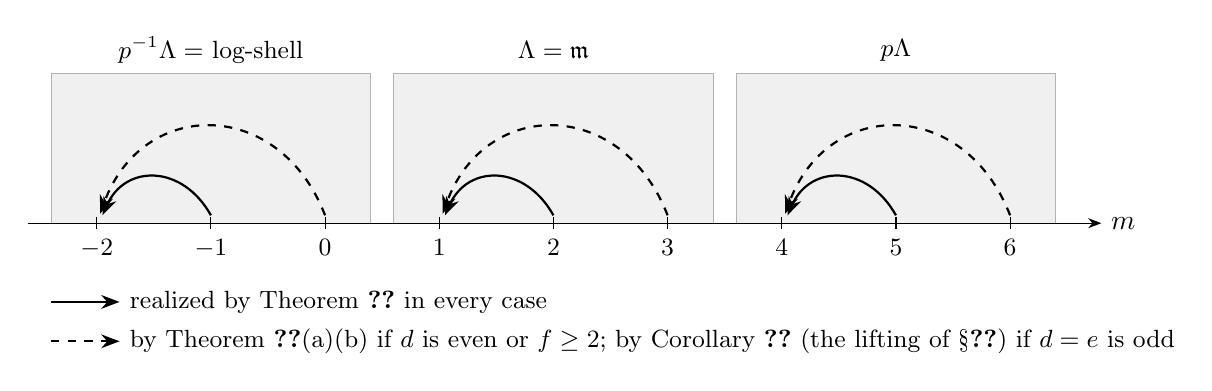
\begin{tikzpicture}[x=1.45cm,y=1cm,>=Stealth]
\foreach \lft/\lab in {-2.4/{$p^{-1}\Lambda=$ log-shell},0.6/{$\Lambda=\fm$},3.6/{$p\Lambda$}}{
  \fill[gray!12] (\lft,0) rectangle ++(2.8,1.9);
  \draw[gray!60] (\lft,0) rectangle ++(2.8,1.9);
  \node[font=\small] at (\lft+1.4,2.2) {\lab};}
\draw[->] (-2.6,0) -- (6.8,0) node[right] {$m$};
\foreach \x in {-2,...,6}{\draw (\x,0.08) -- (\x,-0.08) node[below,font=\small] {$\x$};}
\foreach \s in {-2,1,4}{
  \draw[->,thick] (\s+1,0.1) .. controls (\s+0.75,0.75) and (\s+0.25,0.75) .. (\s+0.05,0.1);
  \draw[->,thick,dashed] (\s+2,0.1) .. controls (\s+1.6,1.6) and (\s+0.4,1.6) .. (\s+0.03,0.12);}
\draw[->,thick] (-2.4,-1.0) -- (-1.8,-1.0) node[right,font=\small]
  {realized by Theorem~\ref{t:exact} in every case};
\draw[->,thick,dashed] (-2.4,-1.5) -- (-1.8,-1.5) node[right,font=\small]
  {by Theorem~\ref{t:exact}(a)(b) if $d$ is even or $f\ge2$; by Corollary~\ref{c:O3} (the lifting of
  \S\ref{s:odd}) if $d=e$ is odd};
\end{tikzpicture}
\caption{The case $e=3$. Within each block of three exponents (a layer $p^q\Lambda$), the images of $\fm^m$ span up to
the outermost lattice $\fm^{\lo(m)}$ of that block. The moves from exponents divisible by $e$ (including
$\cO_K=\fm^0$), drawn dashed, need the lifting of Section~\ref{s:odd} exactly when $d=e$ is odd.}\label{fig:ladder}
\end{figure}

\section{Moving the first generator in odd degree}\label{s:odd}

\subsection{The dichotomy and a reduction}
In this subsection $K$ is small, $d=e\ge3$ is odd and $f=1$. By the periodicity of Proposition~\ref{p:upper} it
suffices to treat $m=0$. Put
\[
\ell_0:=(p\cO+p\Lambda)/p\Lambda\subset\Lambda/p\Lambda .
\]
As $p\cO=\fm^e\supseteq p\fm=p\Lambda$ and $p\cO/p\fm\cong\cO/\fm=\Fp$, the line $\ell_0$ is one-dimensional over
$\Fp$, spanned by the image of $p$ (the image of $\log U^1_{\Qp}=p\Zp$).

\begin{theorem}\label{t:dichotomy}
\tagP\ Exactly one of the following holds.
\begin{enumerate}[label=(\roman*)]
\item Every $\gamma\in\Gamma_K$ preserves $\ell_0$. Then $\gamma(\cO_K)=\cO_K$ for every $\gamma$, and for $e\mid m$
we have $S_K(m)=\fm^m$ and $a_K(m)=0$.
\item Some $\gamma\in\Gamma_K$ does not preserve $\ell_0$. Then for $e\mid m$ we have $S_K(m)=\fm^{m+1-e}$ and
$a_K(m)=e-1$; in particular the images of $\cO_K$ span the log-shell $\fm^{1-e}$.
\end{enumerate}
\end{theorem}
\begin{proof}
The preimage of $\ell_0$ under $\Lambda\to\Lambda/p\Lambda$ is $p\cO$. In case (i), $\gamma$ preserves $p\cO$, hence
$\cO$. In case (ii), for some $\gamma$ we have $\gamma(p)\not\equiv bp\pmod{p\Lambda}$ for all $b\in\Zp$. By
($\Gamma2$), $\Tr(\gamma(p))=\Tr(p)$, so $w:=\gamma(p)-p\in W$, and $w\notin p\Lambda$, that is, $w\notin pW$. By
Lemma~\ref{l:odd}, $\spn\Gamma_K(w)=W$. The module $S_K(e)\supseteq\spn\Gamma_K(p)$ contains $w$ and $p$, hence
$\Lambda$ by Lemma~\ref{l:trace}, and $S_K(e)=\Lambda$ by ($\Gamma1$). Dividing by $p$ gives
$S_K(0)=p^{-1}\Lambda=\fm^{1-e}$.
\end{proof}

For each isomorphism $\phi\colon X\xrightarrow{\sim}G_K$ (Theorem~\ref{t:jw}) let $L_\phi\subset\Lambda/p\Lambda$ be
the line spanned by the image of $y_1^{\phi}:=\log\rec_K^{-1}(\phi(x_1))$ (by Lemma~\ref{l:basis},
$y_1^{\phi}\notin p\Lambda$).

\begin{proposition}\label{p:orbit}
\tagP\ Case (i) of Theorem~\ref{t:dichotomy} holds if and only if $L_\phi=\ell_0$ for every $\phi$. In particular, if
$L_\phi\ne\ell_0$ for one $\phi$, that is, if $y_1^{\phi}\notin\Zp^{\times}p+p\Lambda$, then case (ii) holds.
\end{proposition}
\begin{proof}
For $\alpha\in\Aut(G_K)$, $\alpha\circ\phi$ is again an isomorphism and $L_{\alpha\circ\phi}=\alpha_+(L_\phi)$;
conversely any two isomorphisms differ by an element of $\Aut(G_K)$. So $\{L_\phi\}$ is one $\Gamma_K$-orbit. Suppose
$L_\phi\ne\ell_0$ for some $\phi$. As $\Lambda/p\Lambda=\Fp\yb_1\oplus W/pW$ (Lemma~\ref{l:trace}, in the basis of
$\phi$), we can write $\ell_0=\Fp(\yb_1+\bar w)$ with $\bar w\in W/pW\setminus\{0\}$. The alternating form on $W/pW$
is nondegenerate, so some basis element $v$ of a pair has $\ip{\bar w}v\ne0$. The transvection $T_v$ (or its
inverse) of Proposition~\ref{p:gens}(b) fixes $\yb_1$ and sends $\yb_1+\bar w$ to
$\yb_1+\bar w+\ip{\bar w}v\,v$, which is not an $\Fp$-multiple of $\yb_1+\bar w$ (the coefficient of $\yb_1$ stays
$1$). So case (ii) holds. Conversely, if $L_\phi=\ell_0$ for every $\phi$, the orbit $\{L_\phi\}$ is $\{\ell_0\}$, so
case (i) holds.
\end{proof}

\subsection{Two tools}
From now on $k/\Qp$ is any finite extension of odd degree $d\ge3$ (not necessarily small). Let
$\cG=\mathrm{Gal}(k_{\mathrm{tr}}/k)$ be the tame quotient, $V=V_k$ the wild inertia group, and $V^{(1)}=V$,
$V^{(i+1)}=(V^{(i)})^p[V^{(i)},V]$ its descending $p$-central series (the numbering of \cite{NSW}; the $X^i$ of
\cite{JW} correspond to $V^{(i+1)}$). As $d$ is odd, $\mu_p\not\subset k$, so the character $\alpha$ by which $\cG$
acts on $\mu_{p^s}$ is nontrivial modulo $p$.

Here $s=s(k)$ is the integer such that the maximal tamely ramified extension $k_{\mathrm{tr}}$ of $k$ contains exactly
$p^s$ roots of unity of $p$-power order (the $s$ of the Jannsen--Wingberg presentation \cite[p.~419]{NSW}; $s\ge1$
since $\mu_p\subset k_{\mathrm{tr}}$). If $p\nmid e(k)$, then $s(k)=1$. Indeed, if $s\ge2$, then
$k(\mu_{p^2})\subseteq k_{\mathrm{tr}}$ is tamely ramified over $k$, so its ramification index over $\Qp$ is $e(k)$
times a number prime to $p$; on the other hand it is divisible by the ramification index $p(p-1)$ of $\Qp(\mu_{p^2})$,
so $p\mid e(k)$. In particular $s(K)=1$ for small $K$.

\begin{theorem}[Wingberg's lifting theorem]\label{t:wingberg}
\tagS\ Let $p\ne2$ and $s(k)=1$, and let $\psi_3$ be an automorphism of $G_k/V^{(3)}$ that induces the identity on
$G_k/V$. Then there is an automorphism $\varphi$ of $G_k$ that coincides with $\psi_3$ modulo $V^{(2)}$
\cite[Satz~2]{Wi}, \cite[Thm.~7.5.15]{NSW}, \cite[Prop.~2.6]{Nishio26}.
\end{theorem}

\tagS\ NSW use this theorem to construct nontrivial outer automorphisms of $G_{\Qp}$ \cite[pp.~421--423]{NSW}.
Nishio uses it to construct finite subgroups of $\Aut(G_k)$ acting on the pairs $(x_2,x_3),\dots$
\cite[Prop.~2.6]{Nishio26}. Here we construct an automorphism that preserves the relation itself at the third level
and lift it by this theorem.

\medskip\noindent\tagS\,\tagP\ \textbf{A remark on $s$.} NSW state (7.5.15) with the descending $p$-central series,
after noting that Wingberg's statement was not correct as stated. Nishio states the same theorem, for $s=s(k)$, with the
descending $p^s$-central series $H^{p,i+1,s}=(H^{p,i,s})^{p^s}[H,H^{p,i,s}]$ \cite[Prop.~2.6]{Nishio26}. For $s=1$ the
two agree, and this note uses only this case. For $s\ge2$ the form with the descending $p$-central series cannot be
used. For example (in even degree), for $k=\Qp(\zeta_{p^2})$, where $s=2$, the map $x_1\mapsto x_1x_2$ (the other
generators fixed) gives an automorphism of $G_k/V^{(3)}$ that is the identity on $G_k/V$ (as $x^{p^2}\in V^{(3)}$ and
$[x_1x_2,x_2]\equiv[x_1,x_2]\pmod{V^{(3)}}$). An automorphism of $G_k$ that coincides with it modulo $V^{(2)}$ would
induce the same map on $G_k^{\mathrm{ab}}/p$ (as $V^{(2)}\subseteq G_k^p[G_k,G_k]$), and so would move the line in
$G_k^{\mathrm{ab}}/p$ spanned by the image of the torsion subgroup; but automorphisms of $G_k$ preserve this line, so
no such automorphism exists.

\medskip\noindent\textbf{Notation.} Write $F=F(d+1,\cG)=P\rtimes\cG$, where $P$ is the free pro-$p$ operator group
with operator domain $\cG$ on the free generators $x_0,\dots,x_d$ \cite[p.~74]{JW}. Then $G_k=F/\langle\!\langle
r\rangle\!\rangle$, and $V$ is the image of $P$. Let $P^{(i)}$ be the descending $p$-central series of $P$, and put
$M_1=P/P^{(2)}$, $M_2=P^{(2)}/P^{(3)}$. The group $\cG$ acts from the left by conjugation, $g\cdot x=gxg^{-1}$ (the
convention $y^x=xyx^{-1}$ of \cite{JW}), making both into modules over $R:=\Fp[[\cG]]$; $M_1$ is free on
$\xb_0,\dots,\xb_d$. As $p$ is odd, the $p$-th power gives an $R$-linear map $M_1\to M_2$, and the commutator gives
an alternating bilinear map $B\colon M_1\times M_1\to M_2$ with $B(gu,gv)=g\,B(u,v)$ for $g\in\cG$. Let
$\varepsilon\colon R\to\Fp$ be the augmentation.

\begin{proposition}[the linear part of the relation]\label{p:linear}
\tagS
\begin{enumerate}[label=(\roman*)]
\item The relation $r$ and the Jannsen--Wingberg word $x_1'$ lie in $P$ (Section~\ref{s:jw}).
\item There is $\delta\in R$ with $x_1'\equiv\delta\,\xb_1\pmod{P^{(2)}}$ \cite[2.9]{JW}.
\item The image of the twisted product $(x_0,\tau)$ in $M_1$ is $e'\xb_0$, where $e'$ is the idempotent of
$\Fp[[\langle\tau\rangle]]$ for the component on which $\tau$ acts by $\beta(\tau)^{-1}$, and $e'$ commutes with
$\sigma$ \cite[2.3 and formula (2) on p.~81]{JW}. Hence $e'$ is central in $R$, and the image of $r$ in $M_1$ is
$\theta\,\xb_0$ with $\theta:=-\sigma+\beta(\sigma)^{-1}e'$ (modulo $p$).
\end{enumerate}
\end{proposition}

\subsection{The construction}
\begin{theorem}\label{t:lift}
\tagP\ Let $p$ be an odd prime and $k/\Qp$ a finite extension of odd degree $d\ge3$ with $s(k)=1$ (which always holds
if $p\nmid e$). Fix Jannsen--Wingberg generators and put $y_i=\log\rec_k^{-1}(x_i)$. Then there is an automorphism $\varphi$ of $G_k$ with
\[
\varphi_+(y_1)\equiv y_1+y_2,\qquad\varphi_+(y_i)\equiv y_i\quad(2\le i\le d)\pmod{p\Lambda},
\]
where $\Lambda=\log U^1_k$. In particular $\varphi_+(y_1)\ne y_1$.
\end{theorem}

\begin{proof}
We use the notation of \S6.2.

\emph{(1) The effect of adjusting $x_0$.} For $z\in P^{(2)}$, replacing $x_0$ by $x_0z$ changes $r$ modulo $P^{(3)}$
into $r\cdot\theta\bar z$. Indeed, $z$ is central modulo $P^{(3)}$, so the $x_0$-part
$x_0^{-\sigma}(x_0,\tau)^{\beta(\sigma)^{-1}}$ of $r$ changes linearly in $z$, with the coefficient $\theta$ of
Proposition~\ref{p:linear}(iii); the remaining part $x_1^{p}[x_1,x_1'][x_2,x_3]\cdots$ does not involve $x_0$.

\emph{(2) The character and the ideal.} $\theta R$ is a two-sided ideal of $R$ of codimension $1$. Indeed, $e'$ is a
central idempotent and $\theta R=(1-e')\sigma R+(b-\sigma)e'R=(1-e')R+(b-\sigma)e'R$ with $b=\beta(\sigma)^{-1}\bmod
p$; in $e'R=e'\,\Fp[[\langle\sigma\rangle]]$ the element $b-\sigma$ generates the kernel of the character
$\sigma\mapsto b$. So $\theta R$ is the kernel $I_0$ of the augmentation of the character $\chi_0\colon\sigma\mapsto
b$, $\tau\mapsto\beta(\tau)^{-1}$ (modulo $p$). Since $\beta$ is a lifting of $\alpha$ or of $\alpha^{-1}$ (the
conventions differ: \cite[pp.~74--75]{JW}, \cite[p.~420]{NSW}), $\chi_0=\alpha^{\pm1}\bmod p$. As $d$ is odd,
$\mu_p\not\subset k$, so $\chi_0$ is nontrivial. Extend $g^{\dagger}:=\chi_0(g)g^{-1}$ to an anti-automorphism of $R$.
For $g\in\cG$ we have $B(gu,v)=g\,B(u,g^{-1}v)\equiv\chi_0(g)B(u,g^{-1}v)=B(u,g^{\dagger}v)\pmod{I_0M_2}$, hence
\[
B(au,v)\equiv B(u,a^{\dagger}v)\pmod{I_0M_2}\qquad(a\in R).
\]

\emph{(3) The map.} Choose $\rho_0\in\cG$ with $\chi_0(\rho_0)\ne1$ and put
$c:=(\rho_0-\chi_0(\rho_0))/(1-\chi_0(\rho_0))\in R$. Then $\varepsilon(c)=1$ and $c\in I_0$. Put
$\mu:=-c^{\dagger}(\delta-\delta^{\dagger})$ and $\nu:=-c^{\dagger}\delta c$. As $\varepsilon(c^{\dagger})=\chi_0(c)=0$,
we have $\varepsilon(\mu)=\varepsilon(\nu)=0$. Define the automorphism $\psi$ of $F$ to fix
$\sigma,\tau,x_0,x_2,x_4,\dots,x_d$ and
\[
\psi(x_1)=x_1\cdot w_c,\qquad\psi(x_3)=x_3\cdot w_\mu\,w_\nu ,
\]
where $w_c,w_\mu,w_\nu\in P$ are elements with images $c\,\xb_2$, $\mu\,\xb_1$ and $\nu\,\xb_2$ in $M_1$. As
$\psi$ is unipotent on $M_1$, it is an automorphism of $F$.

\emph{(4) The change of the relation.} Modulo $P^{(3)}$ we have $\psi(r)\,r^{-1}\equiv E$ with $E\in M_2$ equal to
\[
E=p\,c\,\xb_2+B(\xb_1,\delta c\,\xb_2)+B(c\,\xb_2,\delta\xb_1)+B(c\,\xb_2,\delta c\,\xb_2)
+B(\xb_2,\mu\,\xb_1)+B(\xb_2,\nu\,\xb_2)
\]
(here $s=1$; as $p$ is odd, $(uv)^p\equiv u^pv^p$). By the rule of (2) and the alternation of $B$, modulo $I_0M_2$,
\[
E\equiv p\,c\,\xb_2+B\bigl(\xb_2,(c^{\dagger}\delta-c^{\dagger}\delta^{\dagger}+\mu)\xb_1\bigr)
+B\bigl(\xb_2,(c^{\dagger}\delta c+\nu)\xb_2\bigr)=p\,c\,\xb_2\equiv0,
\]
the last step because $c\in I_0$. So $E\in I_0M_2=\theta M_2$, and there is $\zeta\in M_2$ with $\theta\zeta=-E$. Let
$z\in P^{(2)}$ lift $\zeta$, and let $\psi'$ be $\psi$ with $x_0\mapsto x_0z$ instead of $x_0\mapsto x_0$. By (1),
$\psi'(r)\equiv r\pmod{P^{(3)}}$.

\emph{(5) The lifting.} $\psi'$ fixes $\cG$ and preserves the normal closure of $r$ and $P^{(3)}$ (and so does its
inverse). Since $G_k=F/\langle\!\langle r\rangle\!\rangle$ and $V^{(3)}$ is the image of $P^{(3)}$, $\psi'$ induces an
automorphism of $G_k/V^{(3)}$ that is the identity on $G_k/V$. By Theorem~\ref{t:wingberg} there is
$\varphi\in\Aut(G_k)$ that coincides with it modulo $V^{(2)}$.

\emph{(6) Computing $\varphi_+$.} On $V/V^{(2)}$, $\varphi$ acts by $\xb_1\mapsto\xb_1+c\,\xb_2$,
$\xb_3\mapsto\xb_3+\mu\,\xb_1+\nu\,\xb_2$, fixing the other $\xb_i$ ($z\in P^{(2)}$ has no effect). Passing to
$(V/V^{(2)})_{\cG}\cong U^1_k/(U^1_k)^p\cong\Lambda/p\Lambda$ ($\xb_i\mapsto\yb_i$, as in the proof of
Lemma~\ref{l:basis}) gives $\yb_1\mapsto\yb_1+\varepsilon(c)\yb_2=\yb_1+\yb_2$ and
$\yb_3\mapsto\yb_3+\varepsilon(\mu)\yb_1+\varepsilon(\nu)\yb_2=\yb_3$, the other $\yb_i$ being fixed. The action of
$\varphi_+$ modulo $p$ is this map (\S2.2).
\end{proof}

\subsection{Consequences}
\begin{corollary}\label{c:O3}
\tagP\ If $K$ is small, $d=e\ge3$ is odd and $f=1$, then case (ii) of Theorem~\ref{t:dichotomy} holds: some
$\gamma\in\Gamma_K$ does not preserve $\ell_0$, and for $e\mid m$ we have $S_K(m)=\fm^{m+1-e}$ and $a_K(m)=e-1$.
\end{corollary}
\begin{proof}
If $\ell_0=\Fp\yb_1$, the $\varphi$ of Theorem~\ref{t:lift} sends $\yb_1$ to $\yb_1+\yb_2\notin\ell_0$. If
$\ell_0\ne\Fp\yb_1$, the transvection in the proof of Proposition~\ref{p:orbit} moves $\ell_0$.
\end{proof}

\begin{theorem}[main theorem]\label{t:main}
\tagP\ Let $p$ be an odd prime and $K/\Qp$ a finite extension with ramification index $e\le p-2$. Then for every
integer $m$
\[
S_K(m)=\fm_K^{\lo(m)},\qquad a_K(m)=(m-1)\bmod e .
\]
In particular the images of $\cO_K$ span the log-shell $\fm_K^{1-e}$, and if $e\ge2$, then $v_K(\gamma(x))=1-e$ for
some $x\in\cO_K$ and $\gamma\in\Gamma_K$.
\end{theorem}
\begin{proof}
The case $e=1$ is trivial. For $e\ge2$, the only case not covered by Theorem~\ref{t:exact} is $d=e$ odd, $f=1$ and
$e\mid m$, which is Corollary~\ref{c:O3} together with Theorem~\ref{t:dichotomy}(ii) (here $\lo(m)=m+1-e$).
\end{proof}

\begin{corollary}[$(\Qp)_+$ is moved]\label{c:Qp}
\tagP\ Let $p$ be an odd prime and $k/\Qp$ a finite extension of odd degree $d\ge3$ with $s(k)=1$ (not necessarily
small; $s(k)=1$ if $p\nmid e$). Then there is $\alpha\in\Aut(G_k)$ with $\alpha_+\bigl((\Qp)_+\bigr)\cap(\Qp)_+=0$.
\end{corollary}
\begin{proof}
As $d$ is odd, $\mu_p\not\subset k$; the proof of Lemma~\ref{l:basis} goes through, and $y_1,\dots,y_d$ is a
$\Zp$-basis of $\Lambda=\log U^1_k$. By \cite[Thm.~1.3]{Kondo},
$W:=\Lambda\cap\ker\Tr=\langle y_2,\dots,y_d\rangle_{\Zp}$. Write $(\Qp)_+\cap\Lambda=\Zp u$ with $u$ primitive and
$u=c'y_1+w'$ with $c'\in\Zp$, $w'\in W$; as $\Tr(u)\ne0$, $c'\ne0$. (a) If $c'\in\Zp^{\times}$, the $\varphi$ of
Theorem~\ref{t:lift} gives $\varphi_+(u)\equiv u+c'y_2\not\equiv u\pmod{p\Lambda}$. Since $\varphi_+$ preserves the
trace, $\varphi_+(u)\in\Qp u$ would force $\varphi_+(u)=u$, a contradiction. (b) If $c'\in p\Zp$, then $w'\notin pW$,
and some basis element $v$ of a pair has $\ip{w'}v\in\Zp^{\times}$. The transvection $T_v$ of
Proposition~\ref{p:gens}(b) fixes $y_1$, and $T_v(u)=u+\ip{w'}v\,v$; comparing coefficients of $y_1$ shows
$T_v(u)\notin\Qp u$. In both cases the two lines are distinct, so they meet in $0$.
\end{proof}

\begin{remark}[Kondo's question]\label{r:kondo}
\tagP\ The $\varphi$ of Theorem~\ref{t:lift} satisfies $\varphi_+(y_1)\ne y_1$; this is the element whose existence in
odd degree Kondo left open \cite[Rem.~1.10]{Kondo} (answered here for $s(k)=1$; for $s(k)\ge2$ see
Remark~\ref{r:sge2}). In the proof of Kondo's Theorem~1.9 (for even $d_k$ and
absolutely Galois $k$, a representation built from a Lubin--Tate character is not Aut-intrinsically Hodge--Tate) the
parity of the degree enters only through the automorphism $\varphi$ of \cite[Lemma~1.5]{Kondo}, and the property used there is
$\varphi_+\bigl((\Qp)_+\bigr)\cap(\Qp)_+=0$ \cite[proof of Lemma~1.5(2)]{Kondo}. The automorphism of
Corollary~\ref{c:Qp} has this property, so the same proof applies to absolutely Galois $k$ of odd degree $d\ge3$ with
$s(k)=1$. The
conclusion itself was proved by Kondo in a later paper, by an argument with Haar measures that does not produce
explicit automorphisms \cite[Thm.~D]{Kondo26}. What Corollary~\ref{c:Qp} adds is the existence of elements that move
$(\Qp)_+$ itself, and, modulo $p$, the line $\ell_0$.
\end{remark}

\begin{remark}\label{r:explicit}
The $\varphi$ of Theorem~\ref{t:lift} is explicit only modulo $V^{(2)}$; its existence as an automorphism of $G_k$ comes
from Theorem~\ref{t:wingberg}. NSW use the same theorem to construct outer automorphisms of $G_{\Qp}$
\cite[pp.~421--423]{NSW}, and Nishio to construct finite subgroups acting on the pairs $(x_2,x_3),\dots$
\cite[Prop.~2.6]{Nishio26}; those automorphisms fix $x_0$ and $x_1$, so the line of $y_1$ is not moved. Here $x_1$ is
shifted towards $x_2$ at the third level; the commutator terms that this creates are absorbed by $x_3$, the $p$-th
power term and the constraint from the trace by the condition $c\in I_0$ on the twisted augmentation, and the rest by
the adjustment of $x_0$.
\end{remark}

\begin{remark}\label{r:sge2}
\tagH\ For $k$ of odd degree with $s(k)\ge2$ (which occurs only when $p\mid e$; for example, the subfield of degree
$p$ of $\Qp(\zeta_{p^2})$), Theorem~\ref{t:lift} is not proved here. The same construction with the descending
$p^s$-central series, together with the lifting theorem in the form of \cite[Prop.~2.6]{Nishio26}, would presumably
work, but this has not been checked. Version~1.0.0 of this note stated Theorem~\ref{t:wingberg} without the condition
on $s$, and Theorem~\ref{t:lift}, Corollary~\ref{c:Qp} and Remark~\ref{r:kondo} including this case. Since $s=1$ for
small $K$, Theorem~\ref{t:main} and Section~\ref{s:iut} are not affected.
\end{remark}

\section{Application to Step (v) of IUT IV}\label{s:iut}

\subsection{Setting (summary of \cite{Tiers})}
\tagS\ We use the notation of \cite[\S2]{Tiers}. Let $p$ be an odd prime, $j\in\{1,\dots,\ell^{*}\}$ and
$I=\{0,1,\dots,j\}$. For each $i\in I$ let $v_i$ be a place above $p$ (not necessarily distinct),
$k_i=K_{v_i}$, $R_i=\cO_{k_i}$, $e_i$ its ramification index and $\pi_i$ a uniformizer; all factors are assumed
small, so that the different has order $\fd_i=(e_i-1)/e_i$. Put $R_I=\bigotimes_{\Zp}R_i$, let $\tI$ be its
normalization, $T=R_I\otimes\Qp$ and $\fd_I=\sum_i\fd_i$. The element $p^{\lambda}\in k_j$
($\lambda\in\frac1{e_j}\Z$) sits in the factor $j$, and the region is $\Theta=p^{\lambda}\cdot\tI$. The holomorphic
hull $\hull(X)$ of $X\subseteq T$ is the intersection of the sets $c\cdot\tI$ ($c\in T^{\times}$) containing $X$
\cite[Rem.~3.9.5(i)]{IUT3}. The class $\cA$ of the actual (Ind1), (Ind2) consists of the maps $\bigotimes_ic_i\gamma_i$
with $c_i\in\Zp^{\times}$ and $\gamma_i\in\Gamma_{k_i}$ \cite[Def.~2.3]{Tiers}. Put
$U_{\cA}=\bigcup_{g\in\cA}g(\Theta)$.

\cite{Tiers} shows: for the classes of maps that preserve the log-shells the hull is exactly
$p^{\ceil{\lambda}-\fd_I}\cdot\tI$ \cite[Thm.~3.2]{Tiers}; $\hull(U_{\cA})$ is contained in it
\cite[Thm.~4.2]{Tiers}; and equality holds if $\lambda\in\Z$ and every $v_i$ satisfies condition (U), that some
$\gamma\in\Gamma_{K_v}$ and $x\in\cO_{K_v}$ have $|\gamma(x)|=|\pi_v|^{1-e_v}$ \cite[Def.~4.3, Thm.~4.4]{Tiers}. That
note did not prove (U) for $e_v\ge2$, and said nothing for $\lambda\notin\Z$ or for odd degree
\cite[\S4.1, \S8]{Tiers}.

\begin{theorem}\label{t:iut}
\tagP\ If all factors are small, then
\[
\hull(U_{\cA})=p^{\ceil{\lambda}-\fd_I}\cdot\tI ;
\]
that is, the actual (Ind1), (Ind2) reach the exact value of \cite{Tiers}.
\end{theorem}
\begin{proof}
For $i\ne j$, Theorem~\ref{t:main} with $m=0$ gives $x_i\in R_i$ and $\gamma_i\in\Gamma_{k_i}$ with
$v_{k_i}(\gamma_i(x_i))=\lo_{e_i}(0)=1-e_i$ (for $e_i=1$ the identity will do). For the factor $j$ put
$m:=e_j\lambda\in\Z$; Theorem~\ref{t:main} gives $x\in\fm_{k_j}^m$ and $\gamma_j$ with
$v_{k_j}(\gamma_j(x))=\lo_{e_j}(m)$. Write $x=p^{\lambda}x_j$ with $x_j\in R_j$. Then
\[
y:=x_0\otimes\cdots\otimes x_{j-1}\otimes p^{\lambda}x_j\in p^{\lambda}R_I\subseteq\Theta,
\]
and its image under $\bigotimes_i\gamma_i\in\cA$ is a pure tensor of nonzero elements, hence a unit of $T$ whose order
in every component (the $\ord$ of \cite[\S2.1]{Tiers}) is
\[
\sum_{i\ne j}\frac{1-e_i}{e_i}+\frac{\lo_{e_j}(m)}{e_j}=-\sum_{i\ne j}\fd_i+\ceil{\lambda}-\fd_j=\ceil{\lambda}-\fd_I ;
\]
here we used $\lo_{e_j}(m)=e_j\floor{(m-1)/e_j}+1$ and $\floor{(m-1)/e_j}=\ceil{\lambda}-1$. A set $c\cdot\tI$ that
contains a unit $u$ contains $u\cdot\tI$ ($uc^{-1}\in\tI$, and $\tI$ is a ring), so
$\hull(U_{\cA})\supseteq p^{\ceil{\lambda}-\fd_I}\cdot\tI$. The reverse inclusion is \cite[Thm.~4.2]{Tiers}.
\end{proof}

\begin{corollary}\label{c:U}
\tagP\ Condition (U) of \cite{Tiers} holds at every small place.
\end{corollary}
\begin{proof}
(U) says $a_{K_v}(0)=e_v-1$, which is Theorem~\ref{t:main} (trivial for $e_v=1$).
\end{proof}

\begin{example}\label{ex:d109}
\tagN\ The explicit initial $\Theta$-datum D109 of \cite{Cat} has $E_0\colon y^2=x(x-1)(x-a)$ over $F_0=\Q(i)$,
$a=\pi^{29}$ with $\pi=10+3i$, $\ell=7$, $F=F_0(\sqrt{-1},E_0[15])$ and $K=F(E_0[7])$ \cite[\S3]{Cat}. The program of
\cite{Walk} lists six places of $\mathbb V^{\mathrm{bad}}_{\mathrm{mod}}$, above
\[
p=109,\ 21577,\ 6065177,\ 534775081,\ 1174770007439769673,\ 16450055877403724897 .
\]
At the place $w$ of $F_0$ above $109$ we have $\ord_w(a)=29$, and at the other five $\ord_w(1-a)=1$; so the reduction
is split multiplicative over $F_{0,w}=\Qp$ (the tangents at the node are $\pm\sqrt{-1}$, resp.\ $\pm1$, and all six
primes are $\equiv1\bmod4$), with $\ord_w(q)=58$, resp.\ $2$, prime to $105$. By Tate's uniformization the completion
of $K$ is $K_v=\Qp(\mu_{420},q^{1/105})$, totally ramified of degree $105$ over the unramified extension
$\Qp(\mu_{420})$. Hence $e=105$, and $f$ is the order of $p$ modulo $420$: $6,12,4,1,12,4$ respectively. All six
places are small. At five of them $[K_v:\Qp]$ is even and Theorem~\ref{t:exact}(a) applies. At the place above
$534775081\equiv1\pmod{420}$, $K_v=\Qp(q^{1/105})$ has degree $105$ and is totally ramified; there
Theorem~\ref{t:exact} does not reach $e\mid m$, in particular condition (U) ($m=0$), and Corollary~\ref{c:O3} is used.
The table of \cite[\S5]{Tiers} has all factors at the bad place above $109$, where $\lambda=29j^2/7\notin\Z$; by
Theorem~\ref{t:iut}, its column ``exact'' is the value reached by the actual (Ind1), (Ind2).
\end{example}

\begin{remark}\label{r:tiers}
\cite{Tiers} gave as a sufficient condition for (U) that the vector $\eta$ of a transvection $x\mapsto x+\Tr(x)\eta$
lie on the boundary of the log-shell \cite[Prop.~4.5]{Tiers}. Corollary~\ref{c:U} proves (U) without this condition:
the proofs of Section~\ref{s:exact} use transvections together with the maps that mix the pairs, not a single
transvection, and in odd degree with total ramification the lifting of Section~\ref{s:odd}. Theorem~\ref{t:iut} also
covers $\lambda\notin\Z$ (always the case at bad places), about which \cite{Tiers} said nothing. The container of
Step~(v) of IUT~IV remains larger than the exact value by exactly a factor $p$ when $\lambda\notin\Z$
\cite[Cor.~3.3]{Tiers}; this difference does not change the shape of the inequality of IUT~IV.
\end{remark}

\section{Two types that are not small: the cyclotomic boundary and fields unramified over \texorpdfstring{$\mathbb Q_2$}{Q2}}\label{s:other}

Sections~\ref{s:setting}--\ref{s:odd} dealt with small $K$ ($p$ odd, $e\le p-2$). In this section we determine
$S_K(m)$ and $a_K(m)$ for two types that are not small (the remaining types are Question~\ref{q:ram}). The new tool is
that the group of principal units that become $p$-th powers in the unramified extension of degree $p$ is determined
by the group. The proofs in \S\S8.1--8.3 do not use the lifting theorem of Section~\ref{s:odd} (Proposition~\ref{p:unions}(a)
in \S8.4 uses Theorem~\ref{t:lift}). For $p=2$ too, $\alpha_+$ and $\Gamma_K$ are defined as in \S2.2 (Hoshi's
reconstruction is stated for all mixed-characteristic local fields \cite[\S3]{Hoshi}). For $n\ge1$ write
$U^{(n)}:=1+\fm^n$ (so $U^1=U^{(1)}$).

\subsection{An invariant lattice from the unramified extension of degree \texorpdfstring{$p$}{p}}

\begin{lemma}\label{l:CK}
\tagP\ Let $K/\Qp$ be a finite extension ($p$ any prime), let $L$ be the unramified extension of $K$ of degree $p$, and
put
\[
C_K:=U^1_K\cap(L^{\times})^p,
\]
the group of principal units of $K$ that are $p$-th powers in $L$. Then $\gamma(\log C_K)=\log C_K$ for every
$\gamma\in\Gamma_K$.
\end{lemma}
\begin{proof}
The inertia group $I_K$ and the wild inertia group $P_K$ of $G_K$ are group-theoretic \cite[Def.~3.5(iii),
Prop.~3.6]{Hoshi}, so they are preserved by every continuous automorphism $\beta$ of $G_K$. The subgroup $H:=G_L$ is the
inverse image of $p\widehat{\Z}$ under $G_K\to G_K/I_K\cong\widehat{\Z}$, so $\beta(H)=H$. In local class field
theory the inclusion $\iota\colon K^{\times}\to L^{\times}$ corresponds to the transfer $G_K^{\mathrm{ab}}\to
H^{\mathrm{ab}}$ \cite[Lemma~1.7(3)]{Hoshi}. The transfer commutes with isomorphisms of groups, so the multiplicative
actions $\beta_K$, $\beta_L$ that $\beta$ and $\beta|_H$ induce on $K^{\times}$ and $L^{\times}$ (through the
reciprocity maps) commute with $\iota$. They preserve the principal units \cite[Prop.~3.11(i)]{Hoshi}. Let $u\in C_K$
with $\iota(u)=y^p$, $y\in L^{\times}$. Then $y$ is a unit with $\bar y^p=1$ in the residue field, so $y\in U^1_L$, and
$\iota(\beta_K(u))=\beta_L(y)^p\in(L^{\times})^p$, that is, $\beta_K(u)\in C_K$. The same holds for $\beta^{-1}$, so
$\beta_K(C_K)=C_K$. The map $\gamma=\beta_+$ of \S2.2 is the action of $\beta_K$ on $U^1_K$ transported by $\log$, so
$\gamma(\log C_K)=\log C_K$.
\end{proof}

\begin{lemma}\label{l:primary}
\tagP\ Assume $\mu_p\subset K$ and put $e_1:=e/(p-1)$ ($e_1=e$ if $p=2$). Then
\[
C_K=U^{(pe_1)}\,(U^1)^p .
\]
In particular, if $e_1=1$ ($e=p-1$, or $p=2$ and $e=1$), then $(U^1)^p\subseteq U^{(p)}$, so $C_K=U^{(p)}$.
\end{lemma}
This is the classical description of the units that give unramified Kummer extensions (primary elements)
\cite[Ch.~IV, (1.4) and \S1, Exercise~7]{FV}; we include a proof.
\begin{proof}
Put $\rho:=\zeta_p-1$ ($\rho=-2$ if $p=2$). Then $v_K(\rho)=e_1$ and $p/\rho^{p-1}\equiv-1\pmod{\fm}$. For $A\in\cO$
let $u=1+\rho^pA\in U^{(pe_1)}$ and
\[
F_A(X):=\frac{(1+\rho X)^p-u}{\rho^p}=X^p+\frac{p}{\rho^{p-1}}X-A+\sum_{j=2}^{p-1}\binom pj\rho^{\,j-p}X^j .
\]
The middle coefficients have valuation $(j-1)e_1>0$, so $F_A$ is a monic polynomial over $\cO$, and its reduction to
the residue field $\kappa$ is the separable polynomial $X^p-X-\bar A$. This has a root in the extension of $\kappa$ of
degree $p$ (the residue field of $L$), so by Hensel's lemma $F_A$ has a root $\xi\in\cO_L$, and $(1+\rho\xi)^p=u$.
Hence $U^{(pe_1)}\subseteq C_K$; clearly $(U^1)^p\subseteq C_K$. Conversely, for $u\in C_K$, $u=y^p$ with $y\in L$,
the map $\sigma\mapsto\sigma(y)/y\in\mu_p$ gives an injection of $C_K/(U^1)^p$ into $\mathrm{Hom}(\mathrm{Gal}(L/K),
\mu_p)$, which has order $p$ (it does not depend on the choice of the root since $\mu_p\subset K$; for elements of the
kernel $y\in K$, and then $y\in U^1_K$). If $A$ is chosen with $\Tr_{\kappa/\Fp}(\bar A)\ne0$, the corresponding $u$
is not a $p$-th power in $K$: a $p$-th root $w\in K$ would satisfy $v_K(w-1)\ge e_1$, so $w=1+\rho X$ with $X\in\cO$,
and $\bar X$ would be a root in $\kappa$. So the image of $U^{(pe_1)}$ is everything, and $C_K=U^{(pe_1)}(U^1)^p$. If
$e_1=1$, then for $x\in\fm$ we have $v_K(px)\ge e+1=pe_1$ and $v_K(x^p)\ge p$, so $(1+x)^p\in U^{(p)}$.
\end{proof}

\begin{proposition}\label{p:invlat}
\tagP\ If $\mu_p\subset K$, every $\gamma\in\Gamma_K$ preserves $p\Lambda+\fm^{pe_1}$ and $\Lambda+\fm^{e_1}$.
\end{proposition}
\begin{proof}
As $pe_1>e/(p-1)$, $\log U^{(pe_1)}=\fm^{pe_1}$, so $\log C_K=p\Lambda+\fm^{pe_1}$ by Lemma~\ref{l:primary}. The claim
follows from Lemma~\ref{l:CK}, $\Qp$-linearity and $p^{-1}\fm^{pe_1}=\fm^{e_1}$.
\end{proof}

\begin{remark}\label{r:aux}
\tagS\ Constructing a lattice from the group side by means of an auxiliary extension is of the same kind as Hoshi's
group-theoretic reconstruction of $\fm^n$ for $\mathbb Q_3(\zeta_3)$, which uses that the $\log$ of the image of the
norm from $k(\zeta_9)$ is $\fm^3$ \cite[Lemma~1.8(iv), Def.~2.9(ii)]{HoshiTop}. Here the unramified extension and the
transfer (the inclusion) are used. Proposition~\ref{p:invlat} does not follow from the invariance of $\Lambda$
(Proposition~\ref{p:Gamma}) alone.
\end{remark}

\subsection{The cyclotomic boundary}
In this subsection $p$ is an odd prime, $e=p-1$ and $\mu_p\subset K$. Then $K\supseteq\Qp(\zeta_p)$ and
$K/\Qp(\zeta_p)$ is unramified, so $\pi:=\zeta_p-1$ is a uniformizer, and $d=(p-1)f$ is even. Let $\kappa$ be the
residue field.

\begin{lemma}\label{l:cyclolat}
\tagP
\begin{enumerate}[label=(\alph*)]
\item $\fm^2\subset\Lambda\subset\fm$ and $[\fm:\Lambda]=p$; $\Lambda/\fm^2$ consists of the lifts of
$\pi\cdot\ker\Tr_{\kappa/\Fp}$.
\item $\Tr(\Lambda)=p\Zp$.
\item The smallest valuation on $\Lambda\setminus\{0\}$ is $2$ if $f=1$ and $1$ if $f\ge2$ (if $f=1$, then
$\Lambda=\fm^2$).
\item $\gamma(\fm)=\fm$ for every $\gamma\in\Gamma_K$.
\end{enumerate}
\end{lemma}
\begin{proof}
(a) As $2>e/(p-1)=1$, $\log U^{(2)}=\fm^2$. For $z\in\cO$ the terms $(\pi z)^n/n$ of $\log(1+\pi z)$ lie in $\fm^2$ for
$2\le n\le p-1$ and for $n>p$, so $\log(1+\pi z)\equiv\pi\bigl(z+(\pi^{p-1}/p)z^p\bigr)\pmod{\fm^2}$, and
$\pi^{p-1}/p\equiv-1\pmod{\fm}$. The image of $z\mapsto z-z^p$ on the residue field is $\ker\Tr_{\kappa/\Fp}$
(Artin--Schreier), which gives (a). (b) $K/\Qp$ is tamely ramified and $\Tr(\fm^j)=p^{\ceil{j/e}}\Zp$, which is $p\Zp$
for $j=1,2$. (c) follows from (a). (d) By Lemma~\ref{l:primary}, $C_K=U^{(p)}$ and $\log C_K=\fm^p=p\fm$ (as
$e=p-1$); apply Lemma~\ref{l:CK}.
\end{proof}

\begin{lemma}\label{l:cyclobasis}
\tagP\ Choose the Jannsen--Wingberg generators so that condition (0) of Proposition~1.1 of Hoshi--Nishio holds (it
suffices to take the integers $g,h$ there larger than $p$ \cite[Prop.~1.1 and its proof]{HN}), and put
$y_i:=\log\rec_K^{-1}(x_i)$ ($0\le i\le d$). Then $y_1,\dots,y_d$ is a $\Qp$-basis \cite[Lemma~1.3]{HN}, there is
$z\in\Qp y_1$ with $\Zp y_0+\Zp y_1=\Zp z$, and
\[
\Lambda=\Zp z\oplus\bigoplus_{i=2}^{d}\Zp y_i,\qquad \Tr(z)=\Tr(y_i)=0\ (i\ge3),\qquad \Tr(y_2)\in p\Zp^{\times}.
\]
\end{lemma}
\begin{proof}
$P_K$ is normally generated by $x_0,\dots,x_d$, and its image in $G_K^{\mathrm{ab}}$ is $\rec_K(U^1)$, so
$\Lambda=\sum_{i=0}^d\Zp y_i$ (conjugates become equal in the abelianization, and the sum is closed since it is finitely
generated). Abelianizing the relation and taking $\log$ gives $h\,y_0=p\,y_1$ with $h\in\Zp$ (here the $s$ of \S6.2 is
$1$, as $p\nmid e$). As $y_1\ne0$, $h\ne0$, so $y_0\in\Qp y_1$, and $\Zp y_0+\Zp y_1$ has rank $1$, so it is $\Zp z$ for
some $z$. The sum is direct by the linear independence of $y_1,\dots,y_d$. As $d$ is even,
$\ker\Tr=\langle y_1,y_3,\dots,y_d\rangle_{\Qp}$ \cite[Thm.~1.3]{Kondo} (whose proof uses this basis property). By
Lemma~\ref{l:cyclolat}(b), $\Tr(y_2)$ generates $p\Zp$.
\end{proof}
Condition (0) cannot be dropped: for $g=h=1$ the abelianized relation reads $p\xb_1=0$, and $y_1=0$.

\begin{lemma}\label{l:R}
\tagP\ Put $V:=\Lambda/p\Lambda$, write $[x]$ for the class of $x\in\Lambda$, and let $\tau:=\Tr/p\bmod p$ (a linear
form on $V$) and $R:=\fm^p/p\Lambda\subset V$. Then $R$ is preserved by $\Gamma_K$, and $R=\Fp[z]$.
\end{lemma}
\begin{proof}
From $\fm^p=p\fm$ and $[\fm:\Lambda]=p$ we get $\dim R=1$, and from $\Tr(\fm^p)=p^2\Zp$ we get $\tau(R)=0$. Since $\fm$
and $\Lambda$ are preserved (Lemma~\ref{l:cyclolat}(d)), so is $R$. Put $U:=\spn_{\Fp}([y_3],\dots,[y_d])$; then
$\ker\tau=\Fp[z]\oplus U$. If $d=2$, then $U=0$ and we are done. If $d\ge4$, by Kondo $\Gamma_K$ contains elements that
fix $y_1,y_2$ and act on $\langle y_3,\dots,y_d\rangle$ as $\Sp_{d-2}(\Zp)$ \cite[Lemma~3.3]{Kondo26} (they also fix
$z$, as $y_0\in\Qp y_1$). Their reductions modulo $p$ act transitively on $U\setminus\{0\}$, so $U$ has no invariant
line. The projection $\ker\tau\to U$ along $\Fp[z]$ is equivariant for this subgroup, so the image of $R$ is $0$, and
$R=\Fp[z]$.
\end{proof}

\begin{lemma}\label{l:Sr}
\tagP\ If $2\le r\le e$, then $S_K(r)=\Lambda$.
\end{lemma}
\begin{proof}
If $d=2$, then $p=3$, $f=1$, $r=2$ and $\fm^2=\Lambda$. Let $d\ge4$. We have $p\Lambda\subset\fm^p\subset\fm^r\subset
\fm^2\subset\Lambda$. Let $N$ be the $\Fp$-subspace of $V$ spanned by the $\Gamma_K$-orbit of the image of $\fm^r$.
Then $N\supseteq R=\Fp[z]$. As $\Tr(\fm^r)=p\Zp$, $N$ contains an element $x$ with $\tau(x)\ne0$, that is, whose
coefficient $\beta$ of $[y_2]$ is nonzero. The automorphism given by the mixing word $M$ of \S4.3 on the first two
pairs $(x_1,x_2),(x_3,x_4)$ (Lemmas~\ref{l:induce} and~\ref{l:ZHJ}) fixes $x_0$ and $x_1$, acts on $\log$ by
$y_2\mapsto y_2+y_1+y_4$, $y_3\mapsto y_3-y_1-y_4$ ($M^{\mathrm{ab}}=T_{a+d}$), and fixes the other $y_i$. If $\eta$ is
the coefficient of $[y_3]$ in $x$, then $Mx-x=(\beta-\eta)([y_1]+[y_4])$. If $\beta=\eta$, apply first an element that
multiplies the pair $(y_3,y_4)$ by $-1$ (an element of $\Sp_{d-2}(\Zp)$); then the coefficient of the difference is
$2\beta\ne0$ ($p$ odd). Hence $[y_1]+[y_4]\in N$. As $[y_1]\in\Fp[z]\subset N$, also $[y_4]\in N$ (it does not matter
whether the $\alpha$ with $y_1=\alpha z$ is divisible by $p$). As $\Sp_{d-2}(\Fp)$ acts transitively on
$U\setminus\{0\}$, $U\subset N$. Since $N$ contains $\ker\tau=\Fp[z]\oplus U$ and an element with $\tau\ne0$, $N=V$.
Together with $p\Lambda\subset\fm^r\subseteq S_K(r)$ this gives $S_K(r)=\Lambda$.
\end{proof}

\begin{theorem}[the cyclotomic boundary]\label{t:cyclo}
\tagP\ Let $p$ be an odd prime and $K/\Qp$ a finite extension with $e=p-1$ and $\mu_p\subset K$. Write $m=ne+r$ with
$1\le r\le e$. Then
\[
S_K(m)=\fm^m\quad(r=1),\qquad S_K(m)=p^n\Lambda\quad(2\le r\le e),
\]
and hence
\[
a_K(m)=\begin{cases}0&(r=1),\\ r-2=(m-2)\bmod e&(r\ge2,\ f=1),\\ r-1=(m-1)\bmod e&(r\ge2,\ f\ge2).\end{cases}
\]
In particular the images of $\cO_K$ span the log-shell $p^{-1}\Lambda$, and the image of some integral element reaches
its boundary.
\end{theorem}
\begin{proof}
For $r=1$, $\fm^m=p^n\fm$ is preserved (Lemma~\ref{l:cyclolat}(d)). For $r\ge2$, $\fm^m=p^n\fm^r\subseteq p^n\Lambda$
and $p^n\Lambda$ is preserved, so $S_K(m)\subseteq p^n\Lambda$, with equality by Lemma~\ref{l:Sr} and $\Qp$-linearity.
The value of $a_K(m)$ follows from the smallest valuation $ne+w$ on $p^n\Lambda$, with $w$ as in
Lemma~\ref{l:cyclolat}(c); that the valuation of an image actually takes this value follows by the argument of
Section~\ref{s:exact}. The ring $\cO_K=\fm^0$ is the case $n=-1$, $r=e$, and $S_K(0)=p^{-1}\Lambda$ is the log-shell
$(2p)^{-1}\log\cO^{\times}=p^{-1}\Lambda$.
\end{proof}

\begin{example}\label{ex:cyclo}
\tagP\ For $\mathbb Q_3(\zeta_3)$ ($e=2$, $f=1$), $a_K(m)=0$ for every $m$, in agreement with Hoshi's result that $\cO$
and all $\fm^n$ are group-theoretic (Remark~\ref{r:Q2}). For $\mathbb Q_5(\zeta_5)$, $a_K(m)=0,0,1,2$ for $m=1,2,3,4$.
For the unramified extensions of $\mathbb Q_3(\zeta_3)$ with $f\ge2$, $a_K(m)$ is $0$ for odd $m$ and $1$ for even $m$.
\end{example}

\subsection{Fields unramified over \texorpdfstring{$\mathbb Q_2$}{Q2}}

\begin{theorem}\label{t:Q2}
\tagP\ Let $K/\mathbb Q_2$ be a finite unramified extension. Then $\gamma(\fm^m)=\fm^m$ for every $\gamma\in\Gamma_K$
and every integer $m$. Hence $S_K(m)=\fm^m$, $a_K(m)=0$, and $\Gamma_K$ preserves the ring of integers $\cO_K$.
\end{theorem}
\begin{proof}
Here $e=1$, $\mu_2\subset K$ and $e_1=1$. By Lemma~\ref{l:primary}, $C_K=U^{(2)}=1+4\cO_K$, and $\log C_K=4\cO_K=\fm^2$
(as $2>e/(p-1)=1$). By Lemma~\ref{l:CK}, $\fm^2$ is preserved; the claim follows from $\fm^m=2^{m-2}\fm^2$ and
$\mathbb Q_2$-linearity.
\end{proof}

\begin{remark}\label{r:Q2}
\tagS\ For $K=\mathbb Q_2$ and $K=\mathbb Q_3(\zeta_3)$ (and for unramified $K$ with $p$ odd) the log-shell equals the
ring of integers, and Hoshi reconstructs $\cO_K$ and all $\fm^n$ group-theoretically \cite[Thm.~A(ii), Lemma~1.8(i)--(iv),
Def.~2.9, Summary~2.11(ii)]{HoshiTop}. For $K$ unramified over $\mathbb Q_2$ of degree at least $2$, the log-shell does
not equal $\cO_K$ \cite[Thm.~A(ii)]{HoshiTop}, but by Theorem~\ref{t:Q2} every automorphism preserves $\cO_K$. We do
not know whether in this case $G_K$ has automorphisms that do not come from field automorphisms. For $p=2$ and
$\sqrt{-1}\notin K$, no presentation of $G_K$ by generators and relations is known \cite[Rem.~2.22]{Kondo}.
Theorem~\ref{t:Q2} should be read as a constraint on any automorphism. For $2$-adic fields containing $\sqrt{-1}$,
Nishio constructs automorphisms that do not come from field automorphisms \cite[Thm.~1.6]{Nishio25}.
\end{remark}

\subsection{Unions of images}
Instead of the module spanned by the images of a lattice, consider the union of the images itself,
\[
A_K(m):=\bigcup_{\gamma\in\Gamma_K}\gamma(\fm^m)\ \subseteq\ S_K(m).
\]
The holomorphic hull of IUT sees only the spanned module, so this does not affect Section~\ref{s:iut}.

\begin{proposition}\label{p:unions}
\tagP
\begin{enumerate}[label=(\alph*)]
\item Let $K$ be small and $d\ge3$ odd. If $f\ge2$, then $A_K(m)=\fm^{\lo(m)}$ for every $m$. If $f=1$ (so $d=e$),
then $A_K(m)=\fm^{\lo(m)}$ for $e\nmid m$, and for $m=ne$
\[
A_K(ne)=p^{\,n-1}\bigl(\{x\in\Lambda:\Tr(x)\notin p^2\Zp\}\cup p\Lambda\bigr).
\]
\item On the cyclotomic boundary (the setting of Theorem~\ref{t:cyclo}) write $m=ne+r$ with $1\le r\le e$. If $r=1$,
then $A_K(m)=\fm^m$; if $r\ge2$ and $(f,r)\ne(1,e)$, then $A_K(m)=p^n\Lambda$; if $f=1$ and $r=e$, then
\[
A_K(m)=p^n\bigl(\{x\in\Lambda:\Tr(x)\notin p^2\Zp\}\cup\fm^p\bigr).
\]
\item In the case $m=ne$ of (a), and in the case $f=1$, $r=e$, $d\ge4$ of (b), $A_K(m)$ is not an additive group, and
its Haar measure relative to $S_K(m)$ is $1-1/p+p^{-d}$ and $1-1/p+p^{1-d}$ respectively (for example $101/125$ for
$\mathbb Q_5(\zeta_5)$).
\end{enumerate}
\end{proposition}
\begin{proof}
Let $q\colon\Lambda\to V:=\Lambda/p\Lambda$ be the quotient map. For a $\Zp$-submodule $B$ with $p\Lambda\subseteq
B\subseteq\Lambda$ we have $\bigcup_\gamma\gamma(B)=q^{-1}\bigl(\bigcup_\gamma\gamma(q(B))\bigr)$: if $q(x)=\gamma q(b)$
with $b\in B$, then $x-\gamma(b)\in p\Lambda$ and $\gamma^{-1}(x-\gamma(b))\in p\Lambda\subseteq B$, so
$x=\gamma\bigl(b+\gamma^{-1}(x-\gamma(b))\bigr)\in\gamma(B)$. So it suffices to determine the orbits in $V$.

(a) We have $V=\Fp\yb_1\oplus\bar W$ with $\bar W=W/pW$, and $\tau:=\Tr/\Tr(y_1)\bmod p$ is preserved by $\Gamma_K$. The
elements of $\Gamma_K$ that fix $y_1$ and act on $W$ as $\Sp_{d-1}(\Zp)$ \cite[Lemma~3.3]{Kondo26} fix $\yb_1$ and act
transitively on $\bar W\setminus\{0\}$. The $\varphi$ of Theorem~\ref{t:lift} ($s=1$ for small $K$) maps $\yb_1$ to
$\yb_1+\yb_2$. So the orbits in $V$ are $\{0\}$, $\bar W\setminus\{0\}$ and the sets $\tau^{-1}(t)$ ($t\ne0$). For
$1\le r\le e$ the subspace $I_r:=q(\fm^r)$ has dimension $f(e+1-r)$ and $\tau(I_r)=\Fp$. If the dimension is at least
$2$, $I_r$ meets every orbit, the union is $V$, and $A_K(r)=\Lambda$. If it is $1$ ($f=1$, $r=e$), then $I_e=\Fp\bar p$
and the union is $\{0\}\cup\{\tau\ne0\}$. The general case follows from $\fm^{ne+r}=p^n\fm^r$.

(b) $R=\Fp[z]$ and $\tau$ are preserved by $\Gamma_K$ (Lemma~\ref{l:R}). Use coordinates $(t,u)$ on
$V/R=\Fp[y_2]\oplus U$. If $d=2$, then $U=0$, and as $\tau$ is preserved the orbits are points. If $d\ge4$, the $M$ of
the proof of Lemma~\ref{l:Sr} acts modulo $R$ by $(t,u)\mapsto\bigl(t,u+(t-u_3)[y_4]\bigr)$, where $u_3$ is the
coefficient of $[y_3]$ in $u$. The map $u\mapsto u-u_3[y_4]$ is a transvection in the direction $[y_4]$, an element of
$\Sp_{d-2}$, so composing with its inverse gives the translation $(t,u)\mapsto(t,u+t[y_4])$, and conjugating by
$\Sp_{d-2}$ gives $(t,u)\mapsto(t,u+tv)$ for every $v\in U$. So the orbits in $V/R$ are $\{0\}$, $U\setminus\{0\}$ and
$\{t\}\times U$ ($t\ne0$). We have $q(\fm^r)\supseteq R$, and the intersection of $q(\fm^r)/R$ with $\ker\tau$ has
dimension $f(e+1-r)-1$. If this is at least $1$, the union is $V$; if it is $0$ ($f=1$, $r=e$), the union is
$R\cup\{\tau\ne0\}$, and it cannot be larger since all of $\Gamma_K$ preserves $R$ and $\tau$. The inverse image of $R$
is $\fm^p$.

(c) In $V$ the set $\{\tau\ne0\}$ has $(p-1)p^{d-1}$ elements. Add the element $0$ in (a) and the $p$ elements of $R$
in (b), and divide by $p^d$. The union is not an additive group: in (a), $\yb_1$ and $-\yb_1+w$ ($0\ne w\in\bar W$) lie
in it but their sum does not; in (b) the same holds for $[y_2]$ and $-[y_2]+u$ ($0\ne u\in U$).
\end{proof}

\begin{remark}\label{r:EssLgc}
\tagS\ Mochizuki writes that for any $\Zp$-automorphism $\phi$ of the log-shell $\cI_k$ one has
$\phi(U(\cO_k,n))\subseteq\bigcup_{i=-s}^{s}U(\cO_k,n+i)$, where $U(\cO_k,n)$ is the set of elements of $p^n\cO_k$ that
are not in $p^{n+1}\cO_k$, and $s$ depends only on $k$ \cite[Ex.~3.5.1(ii)]{EssLgc}. Proposition~\ref{p:unions}
determines exactly the union of the images of a lattice under the automorphisms of the actual Galois group.
\end{remark}

\section{Relation to earlier work}\label{s:prior}
\begin{itemize}
\item \tagS\ The ring of integers is not group-theoretic. Hoshi states that there are automorphisms of $G_L$ that do
not preserve the ring of integers of $\overline L$, and that no functorial group-theoretic algorithm can reconstruct
$(\cO_k)_+$ uniformly for all mixed-characteristic local fields \cite[Rem.~4.3.1(ii)(iii)]{Hoshi},
\cite[Rem.~2.11.2]{HoshiTop}. Hoshi also shows that the log-shell equals the ring of integers exactly when $p$ is odd and
$k$ is unramified, or $k\cong\mathbb Q_2$ or $\mathbb Q_3(\zeta_3)$ \cite[Thm.~A(ii)]{HoshiTop}, and in these cases
reconstructs the ring of integers and all $\fm^n$ group-theoretically \cite[Def.~2.9, Summary~2.11(ii)]{HoshiTop}. The
present note measures, for each small $K$, how far the ring of integers is moved.
\item \tagS\ Types that are not small (Section~\ref{s:other}). The case $\mathbb Q_3(\zeta_3)$ of
Theorem~\ref{t:cyclo} and the case $\mathbb Q_2$ of Theorem~\ref{t:Q2} are contained in Hoshi's reconstruction above,
and constructing lattices with an auxiliary extension is of the same kind as \cite[Lemma~1.8(iv)]{HoshiTop}
(Remark~\ref{r:aux}). For the cyclotomic boundary with $p\ge5$ or $f\ge2$, and for fields of degree at least $2$
unramified over $\mathbb Q_2$, we have not found an earlier treatment. The description of the units that give
unramified Kummer extensions is classical \cite[Ch.~IV, (1.4) and \S1, Exercise~7]{FV}. For $2$-adic fields containing
$\sqrt{-1}$, Nishio constructs automorphisms that do not come from field automorphisms \cite[Thm.~1.6]{Nishio25}. For
unions of images, Mochizuki writes a bound in the form of a union for any $\Zp$-automorphism of the log-shell
\cite[Ex.~3.5.1(ii)]{EssLgc} (Remark~\ref{r:EssLgc}).
\item \tagS\ Upper bounds. Hoshi's valuation with an indeterminacy \cite[Prop.~1.10(ii)]{HoshiTop} bounds the drop of
the valuation (Remark~\ref{r:hoshi}). The bound of Proposition~\ref{p:upper} comes from the invariance of $\Lambda$
and is of the same kind; the claim here is that it is always attained.
\item \tagS\ Traces and transvections. Hoshi and Nishio prove the preservation of traces and give unipotent induced maps
for abelian extensions of even degree \cite[Lemma~2.3(ii), Thm.~1.5]{HN}. Kondo describes the kernel of the trace by
the generators of the Jannsen--Wingberg presentation \cite[Thm.~1.3]{Kondo}, gives in even degree an automorphism
moving $(\Qp)_+$ \cite[Lemma~1.5]{Kondo}, and shows that $\Sp_{2g}(\Zp)$ lies in the image of the induced maps
\cite[proof of Thm.~2.19]{Kondo}, \cite[Lemma~3.3]{Kondo26}. The maps and arguments of Sections~\ref{s:pairs}
and~\ref{s:exact} are of the same kind; this note combines them on the integral basis to determine the movement of
the lattices.
\item \tagS\ The question in odd degree. Kondo wrote that it was not clear whether an $\alpha$ with
$\alpha_+(y_1)\ne y_1$ exists in odd degree \cite[introduction, Rem.~1.10]{Kondo}. A later paper of Kondo proves, for
nontrivial finite Galois extensions including those of odd degree, that the Lubin--Tate representations are not
Aut-intrinsically Hodge--Tate, by an argument with Haar measures \cite[Thms.~C, D]{Kondo26}; that paper does not
construct elements moving $y_1$ or $(\Qp)_+$, does not refer to Remark~1.10, and notes that explicit automorphisms are
not obtained \cite[remark after Thm.~D, Rem.~3.7]{Kondo26}. Theorem~\ref{t:lift} shows that the element of
Remark~1.10 exists in odd degree when $s(k)=1$ (which always holds if $p\nmid e$).
\item \tagS\ The lifting theorem and the presentation. We use the presentation of Jannsen and Wingberg \cite{JW}, the
computation of the linear part of the relation in Section~2 of their paper, and Wingberg's lifting theorem
\cite[Satz~2]{Wi}, \cite[Thm.~7.5.15]{NSW}. NSW construct nontrivial outer automorphisms of $G_{\Qp}$ with it
\cite[pp.~421--423]{NSW}. Nishio uses the same lifting to construct finite subgroups of $\Aut(G_k)$ acting on the pairs
$(x_2,x_3),\dots$ \cite[Prop.~2.6, Thm.~2.8]{Nishio26}; Nishio states the theorem with the descending
$p^s$-central series, which agrees with the form in NSW in the case $s=1$ used here (the remark after
Theorem~\ref{t:wingberg}). Those automorphisms fix $x_0$ and $x_1$, so they do not move the line of $y_1$, and the
paper does not consider the ring of integers or $(\Qp)_+$. Kumpitsch's Jannsen--Wingberg automorphisms and combinatorial Dehn
twists \cite[Prop.~3.2.4, Thm.~7.5.5]{Ku} and Gropper's arithmetic Dehn twists \cite{Gr} do not concern the movement of
the ring of integers either. For $p=2$, Nishio studies the outer automorphism groups of the absolute Galois groups of
$2$-adic fields \cite{Nishio25}.
\item \tagS\ IUT. The author's note \cite{Tiers} determined the exact hull in Step~(v) and gave condition (U) for the
actual (Ind1), (Ind2) to reach it; Section~\ref{s:iut} continues it. Mochizuki writes that the valuation data ``is
precisely the data that is `deformed' by automorphisms of $k$ that do not arise from field automorphisms''
\cite[\S I3]{AbsTopIII}, describes (Ind1) as arising from automorphisms of $G_k$ that do not in general preserve the
ring structure \cite[\S3.7(i)]{Alien}, writes that ``automorphisms of the $\Zp$-module $I_k$ only give rise to bounded
discrepancies in the orders of nonzero elements of $\cO_k$'' \cite[Ex.~3.5.1]{EssLgc}, and, in an e-mail quoted by
Joshi, that such automorphisms ``can act in a fashion that fails to preserve differents, discriminants'' and other
quantities \cite[Appendix~16]{JoshiAnab}. Scholze and Stix note: ``Such isomorphisms exist for Galois groups of
$p$-adic fields, but this did not seem to enter the discussion in a critical way'' \cite[fn.~4]{SS}. Mochizuki's
formalization report mentions ``a small discrepancy (arising from (Ind1,2,3) + hull)'' \cite[p.~11]{Fm26}. Dupuy and
Hilado treat (Ind1), (Ind2) as acting through the automorphisms of the $\Zp$-lattices of the log-shells
\cite[p.~17, \S4.8]{DH1}; lana-agents/iut uses the group \texttt{tensorAut} of factorwise automorphisms of the
log-shells, which contains the image of $\mathrm{Ism}$ and is described there as a deliberate enlargement
(\lean{Iut/Concrete/LocalConstruct/IndAut.lean}, 11 October 2026), and states that for $\lambda=0$ the hull is exactly
the container of IUT~IV (\lean{Iut/WallEquiv/VcI.md}, 13 October 2026) \cite{lana}. Minamide and Tsujimura prove
$\mathrm{Ism}(G_K)=\Zp^{\times}$ \cite[Thm.~F, Thm.~7.4]{MT}, and write ``Theorem F implies that (Ind2) is relatively small'' \cite{MT}. Takkun-kohinata/IUT\_LEAN states, in a comment of \lean{Thm311.lean}, that (Ind1), (Ind2)
preserve volume and so do not contribute to the volume estimate of the hull (our paraphrase) \cite{Takkun}; this
concerns each image. Zeng computes the index by which the hull enlarges the integral structure of a tensor product of
rings of integers \cite{Zeng}. Joshi reads (Ind1) as anabelomorphy \cite[\S8.11.2]{JoshiIII}, a reading different from
the one used here.
\item \tagP\ What is added here: (1) for small $K$, the determination of $S_K(m)$ and $a_K(m)$ for every $m$; (2) in
odd degree $d\ge3$ with $s(k)=1$, the existence of an automorphism moving $y_1$ (the element of Kondo's Remark~1.10),
and of automorphisms moving $(\Qp)_+$ and, modulo $p$, the line $\ell_0$; (3) for Step~(v) of IUT~IV, the removal of
the hypotheses $\lambda\in\Z$ and (U) of \cite{Tiers}: at small places the actual (Ind1), (Ind2) reach the same hull as
the factorwise automorphisms of the log-shells; (4) an invariant lattice determined by the unramified extension of
degree $p$, and the movement of the lattices on the cyclotomic boundary and for fields unramified over $\mathbb Q_2$
(Section~\ref{s:other}); (5) the unions of images (Proposition~\ref{p:unions}).
\end{itemize}

\section{Remaining questions}\label{s:questions}
What is determined here is the module spanned by the images of the lattices $\fm_K^m$ (and, in some cases, the union
of the images). For the group of induced maps itself, and outside the scope of this note, the following questions
remain.

\begin{question}[the group of induced maps]\label{q:group}
Let $p$ be an odd prime, $K/\Qp$ a finite extension with $\mu_p\not\subset K$, $\Lambda=\log U^1_K$, and
\[
T_K:=\{\,g\in\GL_{\Zp}(\Lambda)\mid\Tr\circ g=\Tr\,\}.
\]
By Proposition~\ref{p:Gamma}, $\Gamma_K\subseteq T_K$ (restricting to $\Lambda$). Is $\Gamma_K=T_K$? If not, is
$\Gamma_K$ an open subgroup of $T_K$? At least, do their images in $\GL(\Lambda/p\Lambda)$ agree?
\end{question}

\begin{remark}[what is known]\label{r:known}
We record what is known.
\begin{itemize}
\item \tagP\ For small $K$, by Theorem~\ref{t:main}, $\Gamma_K$ and $T_K$ give the same modules spanned by the images of
$\fm_K^m$ for every $m$ (both $\fm_K^{\lo(m)}$: $T_K$ preserves $\Lambda$, so the upper bound is the same, and
$\Gamma_K\subseteq T_K$ gives the lower bound). The movement of the lattices does not distinguish the two.
\item \tagP\ In odd degree $d=2g+1\ge3$ with $s(K)=1$, with $W:=\Lambda\cap\ker\Tr$, the image of $\Gamma_K$ in
$\GL(\Lambda/p\Lambda)$ satisfies
\[
(W/pW)\rtimes\Sp_{2g}(\Fp)\ \subseteq\ \mathrm{Im}\ \subseteq\ (W/pW)\rtimes\GL(W/pW),
\]
where $W/pW$ is the group of translations $\yb_1\mapsto\yb_1+w$ (identity on $W/pW$). The left inclusion follows from
Kondo's $\Sp_{2g}(\Zp)\subseteq\Gamma_K$ \cite[Lemma~3.3]{Kondo26} and the conjugates under $\Sp_{2g}$ of the
$\varphi$ of Theorem~\ref{t:lift} (the translation $\yb_1\mapsto\yb_1+\yb_2$ modulo $p$); the right one from the
preservation of the trace.
\item \tagS\ Kondo proves the lower bound $\dim\Gamma_K\ge2g^2+g$ for the dimension as a $p$-adic Lie group
\cite[Lemma~3.3]{Kondo26}; the dimension of $T_K$ is $d^2-d$.
\item \tagH\ The image modulo $p$ presumably reduces, by the method of Section~\ref{s:odd} (automorphisms at the third
level and Theorem~\ref{t:wingberg}), to a computation of the automorphism group of a twisted form over
$\Fp[[\cG]]$. For example, the map moving the pair $(x_2,x_3)$ by $\xb_2\mapsto a\xb_2$,
$\xb_3\mapsto(a^{\dagger})^{-1}\xb_3$ seems to give an element outside $\Sp$ on $W/pW$ when
$\varepsilon(a)\ne\chi_0(a)$, in which case the image would be the whole right-hand side. This has not been checked.
\item \tagS\ For Demu\v{s}kin groups, every automorphism that preserves the cup product and the Bockstein comes from a
group automorphism \cite[Thm.~6.3.2]{Ku}, and Kumpitsch conjectures a surjectivity of the same kind for $G_K$ with
$\mu_{p^t}\subseteq K$ \cite[p.~17]{Ku}. Question~\ref{q:group} is an analogue on the units for $\mu_p\not\subset K$.
\end{itemize}
\end{remark}

\begin{question}[larger ramification]\label{q:ram}
For $p=2$ with $K/\mathbb Q_2$ ramified, or for odd $p$ and $e\ge p$, determine $S_K(m)$ and $a_K(m)$.
\end{question}
The case $e=p-1$ is settled by Remark~\ref{r:pminus1} ($\mu_p\not\subset K$) and Theorem~\ref{t:cyclo}
($\mu_p\subset K$), and the case of fields unramified over $\mathbb Q_2$ by Theorem~\ref{t:Q2}. In the remaining cases
an upper bound again follows from the invariance of $\Lambda=\log U^1_K$, but in general $\Lambda\ne\fm_K$ and the form
changes. If $\mu_p\subset K$, the invariant lattice $\Lambda+\fm^{e_1}$ of Proposition~\ref{p:invlat}
($e_1=e/(p-1)$) can also be used for the upper bound. For odd $p$ and odd degree, Theorem~\ref{t:lift} can be used
when $s(K)=1$. For $p=2$ one has to restart from the tools of Sections~\ref{s:jw}--\ref{s:odd} (the Jannsen--Wingberg
presentation for odd primes); see \cite{Nishio25} for outer automorphisms in the $2$-adic case. We also do not know
whether, for $K$ unramified over $\mathbb Q_2$ of degree at least $2$, $G_K$ has automorphisms that do not come from
field automorphisms (Remark~\ref{r:Q2}).

\begin{question}[an explicit automorphism]\label{q:explicit}
For odd $d\ge3$, give an automorphism of $G_k$ with $\alpha_+(y_1)\ne y_1$ explicitly, as words in the
Jannsen--Wingberg generators.
\end{question}
The $\varphi$ of Theorem~\ref{t:lift} is determined only modulo the second level, and its existence as an automorphism
of $G_k$ comes from the lifting theorem (Theorem~\ref{t:wingberg}), which gives existence and not the form of the
words. Kondo also notes, for a different purpose (automorphisms that destroy the Hodge--Tate property), that explicit
automorphisms are not obtained \cite[Rem.~3.7]{Kondo26}.

\begin{question}[$s\ge2$]\label{q:sge2}
For $k/\Qp$ of odd degree $d\ge3$ with $s(k)\ge2$, is there $\alpha\in\Aut(G_k)$ with $\alpha_+(y_1)\ne y_1$?
\end{question}
This amounts to checking the expectation of Remark~\ref{r:sge2}.

\section{Limitations}
\begin{itemize}
\item The statements about lattices concern only small $K$, $K$ with $e=p-1$ (Remark~\ref{r:pminus1},
Theorem~\ref{t:cyclo}), and $K$ unramified over $\mathbb Q_2$. The cases $p=2$ with $K$ ramified and $p$ odd with
$e\ge p$ (wild ramification) are not treated.
\item $\Gamma_K$ itself is not determined, and the $\varphi$ of Theorem~\ref{t:lift} is explicit only modulo the second
level. Theorem~\ref{t:lift} is proved only for $s(k)=1$ (Remark~\ref{r:sge2}).
\item Theorem~\ref{t:lift} uses as known inputs the presentation of Jannsen and Wingberg with the computations of
Section~2 of their paper, and Wingberg's lifting theorem (NSW (7.5.15)). The proof of the lifting theorem \cite{Wi}
has not been checked here; we rely on the form stated in NSW, who note that the statement in \cite{Wi} was not correct
as stated. This note uses only the case $s=1$, in which the form in NSW agrees with that of \cite[Prop.~2.6]{Nishio26}
(the remark after Theorem~\ref{t:wingberg}).
\item The check in Lean (Section~\ref{s:lean}) is relative: the cited results and some classical facts are hypotheses,
and Lean does not check that these hypotheses state the cited results correctly. Lemma~\ref{l:small}(c)(d),
Remark~\ref{r:pminus1}, Lemma~\ref{l:cyclolat}, the assembly of the automorphism of $G_k$ in Theorem~\ref{t:lift}
(the computation in the presentation and the lifting), and the passage to the holomorphic hull in
Theorem~\ref{t:iut} are not in Lean. The author's own reading of the proofs is still in progress.
\end{itemize}

\section{Machine verification}\label{s:lean}

Many of the \tagP\ statements are checked in Lean~4 (v4.30.0) with Mathlib (v4.30.0). The files are in the folder
\texttt{log-shell-edge/lean} of the deposit (Section~\ref{s:repro}). What is checked is that each statement follows, by
the proof given here, from the hypotheses in the right-hand column of Table~\ref{tab:lean}. The cited results (\tagS)
and the classical facts about local fields that are not in Mathlib are hypotheses of the theorems (fields of
structures), not axioms. Lean does not check that these hypotheses state the cited results correctly. Every theorem
depends on no axioms other than \texttt{propext}, \texttt{Classical.choice} and \texttt{Quot.sound}, and no
\texttt{sorry} and no \texttt{native\_decide} is used; the file \texttt{Verify.lean} of the deposit prints the axioms
of the main results. The README of the folder gives the names of the Lean theorems.

In most files the field $K$ is replaced by a model: a $\Qp$-vector space $V$ with the lattices $L_j=\fm^j$
($L_{j+e}=pL_j$, strictly decreasing), a basis $y$ of $\Lambda=L_1$, the linear form $\tau=\Tr/p$, and a subgroup
$\Gamma$ of linear automorphisms (the maps $\alpha_+$). The multiplication of $K$, the group $G_K$ and the reciprocity
map are not in Lean; what the proofs use about them enters as hypotheses. Only Lemma~\ref{l:small}(a)(b) is proved for
an actual complete ultrametric normed field.

\begin{table}[p]
\centering\small
\begin{tabular}{@{}>{\raggedright\arraybackslash}p{0.2\textwidth}>{\raggedright\arraybackslash}p{0.34\textwidth}>{\raggedright\arraybackslash}p{0.38\textwidth}@{}}
\toprule
Statement & Checked in Lean & Hypotheses\\
\midrule
Lemma~\ref{l:small}(a)(b) & $\mu_p\not\subset K$; $U^1$ is torsion-free; $\log$ is a bijection $U^1\to\fm$ that preserves
norms and is a homomorphism & $\rho^e=\lVert p\rVert$ ($\rho$ the norm of a uniformizer), $e\le p-2$, discreteness ($\lVert
x\rVert<1$ implies $\lVert x\rVert\le\rho$)\\
Proposition~\ref{p:upper} & $S_K(m)\subseteq\fm^{\lo(m)}$ (hence $a_K(m)\le(m-1)\bmod e$), $S_K(m+e)=p\,S_K(m)$,
$a_K(m+e)=a_K(m)$ & ($\Gamma1$)\\
Lemma~\ref{l:basis} & the computation of the $\Zp$-module modulo the relation (if it is torsion-free, the coefficient is a
unit and $y_1,\dots,y_d$ are independent) & the $p$-part of the abelianization of $G_K$ is this module (Theorem~\ref{t:jw}
and the reciprocity map)\\
Lemma~\ref{l:trace} & all & Kondo's description of the kernel of the trace; Lemma~\ref{l:small}(d)\\
Lemma~\ref{l:induce} & that the automorphism descends through the presentation to $X$ & that $\alpha_+$ acts on
$\Lambda$ by the matrix of the abelianization (through the reciprocity map and $\log$)\\
Lemmas~\ref{l:pairs}, \ref{l:ZHJ} & all (identities in free groups, abelianizations) & none\\
Proposition~\ref{p:gens}; the map $M$ of Lemma~\ref{l:Sr} & derived from the conclusion of Lemma~\ref{l:induce} & the
conclusion of Lemma~\ref{l:induce}: an automorphism of the free group fixing $z_1$ and the boundary word is realized
in $\Gamma_K$ by the matrix of its abelianization\\
Lemmas~\ref{l:even}--\ref{l:oddspan}, Theorems~\ref{t:exact}, \ref{t:dichotomy}, Proposition~\ref{p:orbit} (the
direction giving (ii)) & all & $\Lambda=\fm$ with its $\Zp$-basis, ($\Gamma1$), ($\Gamma2$), the dimensions of
$\fm^r/p\fm$, the element of Lemma~\ref{l:small}(d), Kondo's description of the kernel of the trace, the conclusion of
Lemma~\ref{l:induce}; for odd degree and total ramification also $\fm^e/p\fm=\Fp\bar p$\\
Theorem~\ref{t:lift} & the identities in the group ring in steps (2)--(4) and (6) of the proof & Theorem~\ref{t:lift}
itself; the computation in the presentation, $\theta R=I_0$, Proposition~\ref{p:linear} and the lifting
(Theorem~\ref{t:wingberg}) are not in Lean\\
Corollaries~\ref{c:O3}, \ref{c:Qp}, \ref{c:U}, Theorem~\ref{t:main}, Remark~\ref{r:kondo} & all & the hypotheses
above, and Theorem~\ref{t:lift} (for odd degree and total ramification, and for Corollary~\ref{c:Qp} and
Remark~\ref{r:kondo})\\
Theorem~\ref{t:iut} & the identity of orders, and the hull of a set containing a unit & the setting of \cite{Tiers}; the
passage to the container and the holomorphic hull is not in Lean\\
Lemmas~\ref{l:CK}, \ref{l:primary} & the group-theoretic cores (maps commuting with the inclusion, a counting) & the
identification with the groups of principal units, and the transfer\\
Proposition~\ref{p:invlat}, Theorem~\ref{t:Q2} & all & the invariance of $\log C_K$ (Lemmas~\ref{l:CK},
\ref{l:primary})\\
Lemma~\ref{l:cyclobasis} & the computation of the module & \cite[Prop.~1.1, Lemma~1.3]{HN}\\
Lemmas~\ref{l:R}, \ref{l:Sr}, Theorem~\ref{t:cyclo}, Proposition~\ref{p:unions} & all & the lattice facts of
Lemma~\ref{l:cyclolat}, the basis of Lemma~\ref{l:cyclobasis}, the transvections of \cite[Lemma~3.3]{Kondo26}, the
conclusion of Lemma~\ref{l:induce}; for Proposition~\ref{p:unions}(a) the hypotheses on small fields and
Theorem~\ref{t:lift}\\
\bottomrule
\end{tabular}
\caption{What is checked in Lean, and what is taken as a hypothesis.}\label{tab:lean}
\end{table}

Not in Lean are Lemma~\ref{l:small}(c)(d), Remark~\ref{r:pminus1}, Lemma~\ref{l:cyclolat}, Examples~\ref{ex:d109}
and~\ref{ex:cyclo}, Remark~\ref{r:known}, and the parts marked ``not in Lean'' in Table~\ref{tab:lean}.

It is also checked in Lean that the maps that the proofs put into $\Gamma$ (those of Proposition~\ref{p:gens}, $M$, the
map of Theorem~\ref{t:lift}, Kondo's transvections) preserve the trace; so these maps do not contradict ($\Gamma2$).
The conclusion of Lemma~\ref{l:induce} is not checked in this way for every automorphism of the free group.

The automorphisms $Z,H,J,M$ of the free group in \S4.3, the two module lemmas used in Lemmas~\ref{l:basis}
and~\ref{l:even}, and the logarithm series over $\Qp$ and over complete ultrametric normed fields are adapted from an
earlier, unpublished Lean development of the author (the comments were rewritten, the namespaces renamed and unused
statements removed).

\section{Reproducibility}\label{s:repro}
The folder \texttt{log-shell-edge/} of the repository \url{https://github.com/turahigashi/iut-explicit-initial-theta}
(tag \texttt{v0.27.0}), also deposited with this note, contains the Lean files of Section~\ref{s:lean} (folder
\texttt{lean}, with \texttt{Verify.lean} and a README), and scripts in Python (standard library only, except that the
last one uses the program of \cite{Walk}, which needs sympy) with their outputs. The checks do not replace the
proofs.
\begin{itemize}
\item \texttt{check\_free\_group.py}: the identities of Section~\ref{s:pairs} in the free group ($Z,H,J$ and the swap of
pairs with their inverses, the preservation of the boundary words, $M(a)=a$) and the matrices of the abelianizations
($Z^{\mathrm{ab}}=T_{d-b}$, $M^{\mathrm{ab}}=T_{a+d}$, the formula for $U_d$).
\item \texttt{check\_lemma52.py}: for $d=2,4,\dots,12$ and random integral $x$, the determinant of the $d$ vectors of
Lemma~\ref{l:even} is $-u^d$.
\item \texttt{check\_group\_ring.py}: steps (2)--(4) and (6) of the proof of Theorem~\ref{t:lift} in finite models. For
eleven metacyclic groups of order $4$ to $27$ (abelian and non-abelian) and all their nontrivial characters $\chi_0$
over $\Fp$ ($25$ pairs), it checks that $e'$ is a central idempotent, that $\theta R=R\theta=I_0$, the adjoint rule,
that $\varepsilon(c)=1$, $c\in I_0$ and $\varepsilon(\mu)=\varepsilon(\nu)=0$, and, for random $\delta$, that $E$ lies
in $I_0M_2$ and that $\theta\zeta=-E$ is solvable, where $M_2=M_1\oplus\Lambda^2M_1$ models the second level of a free
pro-$p$ group; $E$ itself is nonzero in every trial, so without the adjustment of $x_0$ the relation is not preserved
at the third level.
\item \texttt{check\_boundary\_lattices.py}: the lattice facts of Section~\ref{s:other} (Lemma~\ref{l:cyclolat}(a)--(c),
the case $e_1=1$ of Lemma~\ref{l:primary}, $\log U^{(2)}=\fm^2$, the values of $a_K$ in Theorem~\ref{t:cyclo} and
Example~\ref{ex:cyclo}, and the log-shell of fields unramified over $\mathbb Q_2$) for $\Qp(\zeta_p)$ ($p=3,5,7$), the
unramified extensions of degree $2$ and $3$ of $\mathbb Q_3(\zeta_3)$, the unramified quadratic extension of
$\mathbb Q_5(\zeta_5)$ and the fields unramified over $\mathbb Q_2$ of degree $1,2,3$, by exact integer arithmetic
modulo $p^{10}$.
\item \texttt{check\_boundary\_orbits.py}: the orbit computations of Lemmas~\ref{l:R}, \ref{l:Sr} and
Proposition~\ref{p:unions}, in models over $\Fp$ generated only by the elements whose action is stated in the text
(the transvections of $\Sp$, $M$ and $\varphi$): for (b), $(p,d)=(3,2),(3,4),(5,4),(3,6),(7,6)$ and every value of the
$\alpha$ with $y_1=\alpha z$; for (a), $(p,d)=(3,3),(5,3),(7,3),(5,5),(7,5)$.
\item \texttt{example\_d109.py}: the data of Example~\ref{ex:d109}, read from the program \texttt{iut\_compute.py} of
\cite{Walk} (folder \texttt{iut-walkthrough/program} of the same repository).
\end{itemize}

\section*{Changes in version 1.1.0}
Version~1.0.0 of this note is dated 8 November 2026 and has the DOI
\href{https://doi.org/10.5281/zenodo.24050445}{10.5281/zenodo.24050445}. Version~1.1.0 (9 November 2026) differs
from it as follows.
\begin{enumerate}[label=(\arabic*)]
\item Correction of scope. Version~1.0.0 stated Theorem~\ref{t:wingberg} (Wingberg's lifting theorem) without a
condition on $s(k)$, and Theorem~\ref{t:lift}, Corollary~\ref{c:Qp} and Remark~\ref{r:kondo} for every $k$ of odd
degree. The form stated in NSW uses the descending $p$-central series and cannot be used when $s(k)\ge2$ (the remark
after Theorem~\ref{t:wingberg}). The proof works when $s(k)=1$, which holds whenever $p\nmid e$, and these statements
are now restricted to that case; the case $s(k)\ge2$ is Remark~\ref{r:sge2} and Question~\ref{q:sge2}. Since $s=1$
for small $K$, the main theorem (Theorem~\ref{t:main}) and Section~\ref{s:iut} are unchanged.
\item A new Section~\ref{s:other} on two types that are not small: an invariant lattice from the unramified extension
of degree $p$, the cyclotomic boundary, fields unramified over $\mathbb Q_2$, and unions of images; with two new
scripts.
\item A new Section~\ref{s:lean} on the check in Lean~4; the Lean files are in the deposit.
\item Accordingly the abstract, Section~1, the relation to earlier work, the remaining questions, the limitations, the
reproducibility section, the disclosure and the bibliography ([FV] added; for [HN] the revised version of June 2022 is
used) were revised. The former Sections~8--10 are now Sections~9--11, and the former Section~11 is now
Section~\ref{s:repro}.
\end{enumerate}

\section*{Disclosure}
The question studied here arose in the author's discussions with generative AI tools, and the author decided to make it
the subject of this note. The proofs were found with generative AI tools (large language models) under the author's
direction, and these tools were also used for the computations, the formalisation in Lean, the literature search and
the writing. Section~\ref{s:lean} says what is checked in Lean and under which hypotheses; the correspondence between
these hypotheses and the cited results is not checked by Lean. The author's own reading of the proofs is still in
progress. The author takes full responsibility for the note.

\begin{thebibliography}{JoshiAnab}\raggedright
\bibitem[AbsTopIII]{AbsTopIII}
Shinichi Mochizuki, \emph{Topics in absolute anabelian geometry III: global reconstruction algorithms}, version of
November 2015.

\bibitem[Alien]{Alien}
Shinichi Mochizuki, \emph{The mathematics of mutually alien copies: from Gaussian integrals to inter-universal
Teichm\"uller theory}, RIMS K\^oky\^uroku Bessatsu, preprint version.

\bibitem[Cat]{Cat}
Toshihisa Urahigashi, \emph{Explicit initial $\Theta$-data and the two readings of Step (v) of IUT IV, Theorem 1.10:
a catalogue}, version 1.2.0, Zenodo, 2026, \href{https://doi.org/10.5281/zenodo.24039374}{doi:10.5281/zenodo.24039374}.

\bibitem[DH1]{DH1}
Taylor Dupuy and Anton Hilado, \emph{The statement of Mochizuki's Corollary 3.12, initial theta data, and the first two
indeterminacies}, arXiv:2004.13228v1, 28 April 2020.

\bibitem[EssLgc]{EssLgc}
Shinichi Mochizuki, \emph{On the essential logical structure of inter-universal Teichm\"uller theory in terms of
logical AND ``$\wedge$''/logical OR ``$\vee$'' relations: report on the occasion of the publication of the four main
papers on inter-universal Teichm\"uller theory}, March 2024.

\bibitem[Fm26]{Fm26}
Shinichi Mochizuki, \emph{On the formalization of IUT: a preliminary progress report} [joint work in progress with
Y.~Hoshi, G.~Yamashita, Y.~Yang, \dots], April 2026.

\bibitem[FV]{FV}
Ivan B. Fesenko and Sergei V. Vostokov, \emph{Local Fields and Their Extensions}, 2nd ed., Translations of
Mathematical Monographs 121, American Mathematical Society, 2002.

\bibitem[Gr]{Gr}
Nadav Gropper, \emph{Surfaces and $p$-adic fields}, DPhil thesis, University of Oxford, 2022; see also
\emph{Surfaces and $p$-adic fields I: Dehn twists}, arXiv:2303.04309v1, 8 March 2023.

\bibitem[HN]{HN}
Yuichiro Hoshi and Yu Nishio, \emph{On the outer automorphism groups of the absolute Galois groups of
mixed-characteristic local fields}, RIMS Preprint 1931, November 2020 (revised June 2022); Res. Number Theory
\textbf{8} (2022), no.~56.

\bibitem[Hoshi]{Hoshi}
Yuichiro Hoshi, \emph{Introduction to mono-anabelian geometry}, RIMS Preprint 1868, January 2017.

\bibitem[HoshiTop]{HoshiTop}
Yuichiro Hoshi, \emph{Topics in the anabelian geometry of mixed-characteristic local fields}, Hiroshima Math. J.
\textbf{49} (2019), 323--398.

\bibitem[IUT3]{IUT3}
Shinichi Mochizuki, \emph{Inter-universal Teichm\"uller theory III: canonical splittings of the log-theta-lattice},
Publ. Res. Inst. Math. Sci. \textbf{57} (2021), 403--626.

\bibitem[IUT4]{IUT4}
Shinichi Mochizuki, \emph{Inter-universal Teichm\"uller theory IV: log-volume computations and set-theoretic
foundations}, Publ. Res. Inst. Math. Sci. \textbf{57} (2021), 627--723.

\bibitem[JoshiAnab]{JoshiAnab}
Kirti Joshi, \emph{On Mochizuki's idea of anabelomorphy and its applications}, arXiv:2003.01890v7, 21 June 2026.

\bibitem[JoshiIII]{JoshiIII}
Kirti Joshi, \emph{Construction of arithmetic Teichm\"uller spaces III: a `Rosetta Stone' and a proof of Mochizuki's
Corollary 3.12}, arXiv:2401.13508v4, February 2025.

\bibitem[JW]{JW}
Uwe Jannsen and Kay Wingberg, \emph{Die Struktur der absoluten Galoisgruppe $\mathfrak p$-adischer Zahlk\"orper},
Invent. Math. \textbf{70} (1982), 71--98, \href{https://doi.org/10.1007/BF01393199}{doi:10.1007/BF01393199}.

\bibitem[Kondo]{Kondo}
Kaiji Kondo, \emph{Anabelian aspects of the outer automorphism groups of the absolute Galois groups of
mixed-characteristic local fields}, arXiv:2512.09231v2, 12 December 2025.

\bibitem[Kondo26]{Kondo26}
Kaiji Kondo, \emph{Lubin--Tate representations over nontrivial finite Galois extensions of $\Qp$ are not
Aut-intrinsically Hodge--Tate}, arXiv:2605.25428 (v1 25 May 2026, v2 24 September 2026).

\bibitem[Ku]{Ku}
Theresa Kumpitsch, \emph{Outer automorphisms of the absolute Galois group of local fields of mixed characteristic},
Dissertation, Goethe-Universit\"at Frankfurt am Main, 2022.

\bibitem[lana]{lana}
Project LANA, \emph{lana-agents/iut}, Lean repository, \url{https://github.com/lana-agents/iut}, commit
\texttt{553076a} (3 November 2026). Files cited: \lean{Iut/Concrete/LocalConstruct/IndAut.lean} (11 October 2026),
\lean{Iut/WallEquiv/VcI.md} (first committed 13 October 2026).

\bibitem[MT]{MT}
Arata Minamide and Shota Tsujimura, \emph{Anabelian geometry for Henselian discrete valuation fields with quasi-finite
residues}, RIMS Preprint 1973, June 2023.

\bibitem[Nishio25]{Nishio25}
Yu Nishio, \emph{On the outer automorphism groups of the absolute Galois groups of $2$-adic local fields},
arXiv:2512.05095v1, 4 December 2025.

\bibitem[Nishio26]{Nishio26}
Yu Nishio, \emph{Finite subgroups of outer automorphism groups of the absolute Galois groups of mixed-characteristic
local fields}, arXiv:2609.19696v1, 17 September 2026.

\bibitem[NSW]{NSW}
J\"urgen Neukirch, Alexander Schmidt and Kay Wingberg, \emph{Cohomology of Number Fields}, 2nd ed., Grundlehren der
mathematischen Wissenschaften 323, Springer, 2008; electronic edition 2.3 (May 2020), Chapter~VII, \S5, pp.~409--423.

\bibitem[SS]{SS}
Peter Scholze and Jakob Stix, \emph{Why abc is still a conjecture}, 2018.

\bibitem[Takkun]{Takkun}
Takkun-kohinata, \emph{IUT\_LEAN}, Lean repository, \url{https://github.com/Takkun-kohinata/IUT_LEAN}, 15 July 2026.

\bibitem[Tiers]{Tiers}
Toshihisa Urahigashi, \emph{Three tiers of indeterminacy: the exact hull at small places and the container of Step (v)
of IUT IV}, version 1.0.0, Zenodo, 2026, \href{https://doi.org/10.5281/zenodo.24043000}{doi:10.5281/zenodo.24043000}.

\bibitem[Walk]{Walk}
Toshihisa Urahigashi, \emph{A programmer's walkthrough of inter-universal Teichm\"uller theory}, version 1.2.0, Zenodo,
2026, \href{https://doi.org/10.5281/zenodo.24039375}{doi:10.5281/zenodo.24039375}.

\bibitem[Wi]{Wi}
Kay Wingberg, \emph{Der Eindeutigkeitssatz f\"ur Demu\v{s}kinformationen}, Invent. Math. \textbf{70} (1982),
99--113, \href{https://doi.org/10.1007/BF01393200}{doi:10.1007/BF01393200}.

\bibitem[Zeng]{Zeng}
Chunping Zeng, \emph{An integral-structure inflation in the hull operation of IUT Corollary 3.12}, Zenodo, 2026,
first version 29 October 2026, \href{https://doi.org/10.5281/zenodo.23754276}{doi:10.5281/zenodo.23754276}.
\end{thebibliography}
\end{document}
